\documentclass[11pt,a4paper]{article}

\usepackage{amssymb}
\usepackage{amsmath}
\usepackage{lineno} 
\usepackage{dsfont}
\usepackage{amsfonts}
\usepackage{amsthm}
\usepackage{mathtools}
\usepackage{tikz}
\usetikzlibrary{shapes.geometric, arrows}
\usepackage{multirow}
\usepackage{physics}
\usepackage{graphicx}
\usepackage{caption}
\usepackage{subcaption}
\usepackage{listings}
\usepackage{relsize}
\usepackage{bigints}
\usepackage{natbib}
\usepackage[export]{adjustbox}
\usepackage[linesnumbered,commentsnumbered,ruled,vlined]{algorithm2e}
\usepackage[normalem]{ulem}
\usepackage{longtable}
\usepackage{float}
\usepackage{soul}
\usepackage{xcolor}
\usepackage{authblk}

\graphicspath{{figures/}}

\setlength{\textheight}{24.0cm}
\setlength{\textwidth}{16.0cm}
\setlength{\parindent}{0.0cm}
\setlength{\topmargin}{-1.0cm}
\setlength{\oddsidemargin}{0.0cm}
\renewcommand{\baselinestretch}{1.}
\numberwithin{equation}{section}

% Title footnote command
\newcommand\funding[1]{\protect\\ \hspace*{15.37pt}{\bfseries Funding:} #1}
\newcommand\samethanks[1][\value{footnote}]{\footnotemark[#1]}

% Keywords command
\providecommand{\keywords}[1]
{
	\small	
	\textbf{\textit{Keywords---}} #1
}

\title{Modelling the influence of rhizodeposits on root water uptake}

\author[1]{Andrew Mair\thanks{amair@neiker.eus, ORCID: 0000-0003-3847-5215}}
\author[1]{Emma Gomez Peral\thanks{egomez@neiker.eus}}
\author[2]{Mariya Ptashnyk\thanks{m.ptashnyk@hw.ac.uk, ORCID: 0000-0003-4091-5080}}
\author[1,3]{Lionel Dupuy\thanks{ldupuy@neiker.eus, ORCID: 0000-0001-5221-9037}}

\affil[1]{Department of Conservation of Natural Resources, NEIKER, Derio, Basque Country, 48160, Spain}
\affil[2]{School of Mathematical and Computer Sciences, Heriot-Watt University, Edinburgh, Scotland, EH14 4AP, United Kingdom}
\affil[3]{Ikerbasque, Basque Foundation for Science, Bilbao, Basque Country, 48009, Spain}

\date{} 

\begin{document}

\maketitle
\thispagestyle{empty}
\newpage	
\clearpage
\pagenumbering{arabic}
	
\begin{abstract} 
	Previous experimental research has found that the chemical compounds produced by plant roots, referred to generally as rhizodeposits, affect several soil hydraulic properties. For example, the surface tension of soil water, and the contact angle between menisci and the pore surface. What remains less clear is how these effects manifest when considering the water infiltration and retention in the soil, and the consequent impact on the availability of water for uptake by plant roots. By modifying the Richards equation, a novel model for soil water transport was developed which incorporates the influences of rhizodeposits. The finite-element method was used to obtain simulations from the model and calibration against experimental data was achieved through Bayesian optimization. By considering a range of boundary conditions at the upper soil surface, simulations were run to investigate the effects of rhizodeposits on root water uptake under various precipitation regimes. It was found that the overall impact of rhizodeposits on water availability and root water uptake can be positive or negative depending on precipitation regime and root system maturity.  This, therefore, suggests that rhizodeposit characteristics may require consideration when developing crops for improved water use efficiency and stress-resilience.
\end{abstract}

\keywords{Rhizodeposits, Water Infiltration, Modelling, Water Use Efficiency}

\linenumbers

\clearpage

{\scriptsize
\begin{longtable}[h!]{{||p{1.5cm}|p{6cm}|p{1.5cm}|p{6cm}||}}
	\hline
	\rule{0pt}{8pt}
	\textbf{Term} & \textbf{Description} & \textbf{Value} & \textbf{Reference}\\
	\hline
	\rule{0pt}{8pt}
	$c_d$ & Concentration of rhizodeposits dried to soil surface~(mgmg$^{-1}$) & n/a & n/a\\
	\hline
	\rule{0pt}{8pt}
	$c_{d, 0}$ & Initial concentration of rhizodeposits dried to soil surface~(mgmg$^{-1}$) & n/a & n/a\\
	\hline
	\rule{0pt}{8pt}
	$c_w$ & Concentration of rhizodeposits in solution~(mgcm$^{-3}$) & n/a & n/a\\
	\hline
	\rule{0pt}{8pt}
	$c_{w,0}$ & Initial concentration of rhizodeposits in solution~(mgcm$^{-3}$) & n/a & n/a\\
	\hline
	\rule{0pt}{8pt}
	$D_w$ & Rhizodeposit diffusion coefficient~(cm$^2$d$^{-1}$) & 0.65 & \citep{scott1995mathematical}\\
	\hline
	\rule{0pt}{8pt}
	ET$_0$ & Reference evapotranspiration~(cmd$^{-1}$) & 0.1 & \citep{allen1998crop}\\
	\hline
	\rule{0pt}{8pt}
	$f$ & Rhizodeposit release rate~(mgcm$^{-3}$d$^{-1}$) &  n/a & n/a\\
	\hline
	\rule{0pt}{8pt}
	f$_\text{c}$ & Fraction of soil surface covered by vegetation (-) (appears in~K$_\text{e}$) & 0.1 & \citep[Chapter 7, Table 21]{allen1998crop}\\
	\hline
	\rule{0pt}{8pt}
	f$_\text{w}$ & Fraction of soil surface wetted by precipitation (-) (appears in~K$_\text{e}$) & 1.0 & \citep[Chapter 7,Table 20]{allen1998crop}  \\
	\hline
	\rule{0pt}{8pt}
	$g_0$ & Water flux at upper soil surface~(cmd$^{-1}$) & n/a & n/a\\
	\hline
	\rule{0pt}{8pt}
	$g_L$ & Water flux at lower soil surface~(cmd$^{-1}$) & n/a & n/a\\
	\hline
	\rule{0pt}{8pt}
	$h$ & Soil water pressure head~(cm) & n/a & n/a\\
	\hline
	\rule{0pt}{8pt}
	$h_0$ & Initial pressure head condition~(cm) & n/a & n/a\\
	\hline
	\rule{0pt}{8pt}
	$h_1$ & Pressure head associated with anaerobiosis due to soil saturation (cm) (appears in~$\alpha_f$) & 0 & \citep[Table 5]{wesseling1991meerjarige} \\
	\hline
	\rule{0pt}{8pt}
	$h_2$ & Upper limit of pressure head interval in which uptake capacity is maximised (cm) (appears in~$\alpha_f$) & -1.0 & \citep[Table 5]{wesseling1991meerjarige}\\
	\hline
	\rule{0pt}{8pt}
	$h_3$ & Lower limit of pressure head interval in which uptake capacity is maximised (cm) (appears in~$\alpha_f$) & -500.0 & \citep[Table 5]{wesseling1991meerjarige}\\
	\hline
	\rule{0pt}{8pt}
	$h_4$ & Pressure head associated with plant wilting point (cm) (appears in~$\alpha_f$) & -16000.0 & \citep[Table 5]{wesseling1991meerjarige}\\
	\hline
	\rule{0pt}{8pt}
	$h_\Delta$ & Pressure head at hysteresis reversal point~(cm) & n/a & \citep{kool1987development}\\
	\hline
	\rule{0pt}{8pt}
	$K$ & Hydraulic conductivity~(cmd$^{-1}$) & n/a & \citep{mualem1976new,van1980closed}\\
	\hline
	\rule{0pt}{8pt}
	K$_e$ & Evaporation coefficient~(-) & n/a & \citep{allen1998crop,mair2023can}\\
	\hline
	\rule{0pt}{8pt}
	$K_r$ & Effective hydraulic conductivity~(-) & n/a & \citep{mualem1976new,van1980closed}\\
	\hline
	\rule{0pt}{8pt}
	$K_s$ & Hysteretic saturated hydraulic conductivity~(cmd$^{-1}$) & n/a & \citep{vogel1996hydrus}\\
	\hline
	\rule{0pt}{8pt}
	$K_s^d$ & Saturated hydraulic conductivity of drying hydraulic conductivity curve~(cmd$^{-1}$) & n/a & \citep{vogel1996hydrus}\\
	\hline
	\rule{0pt}{8pt}
	$K_{s,0}^d$ & Saturated hydraulic conductivity of drying hydraulic conductivity curve in absence of rhizodeposits~(cmd$^{-1}$) & 120 & \citep{vogel1996hydrus}\\
	\hline
	\rule{0pt}{8pt}
	$K_s^w$ & Saturated hydraulic conductivity of wetting hydraulic conductivity curve~(cmd$^{-1}$) & n/a & \citep{vogel1996hydrus}\\
	\hline
	\rule{0pt}{8pt}
	$K_{s,0}^w$ & Saturated hydraulic conductivity of wetting hydraulic conductivity curve in absence of rhizodeposits~(cmd$^{-1}$) & 72 & \citep{vogel1996hydrus}\\
	\hline
	\rule{0pt}{8pt}
	$K_\Delta$ & Hydraulic conductivity at hysteresis reversal point~(cmd$^{-1}$) & n/a & \citep{vogel1996hydrus}\\
	\hline
	\rule{0pt}{8pt}
	$K^*$ & Fictitious hysteresis parameter in hydraulic conductivity~(cmd$^{-1}$) & n/a & \citep{vogel1996hydrus}\\
	\hline
	\rule{0pt}{8pt}
	K$_{\text{cb}}$ & Basal crop coefficient~(-) & n/a & \citep{allen1998crop}\\
	\hline
	\rule{0pt}{8pt}
	K$_\text{cmax}$ & Maximum crop coefficient (-) (appears in~K$_\text{e}$) & 1.30 & \citep[Chapter 7, Table 19]{allen1998crop}\\
	\hline
	\rule{0pt}{8pt}
	$l$ & Pore tortuosity parameter in hydraulic conductivity function~(-) & $0.5$ & \citep{van2011hydraulic}\\
	\hline
	\rule{0pt}{8pt}
	$L$ & Soil depth~(cm) & 53 & n/a\\ 		
	\hline
	\rule{0pt}{8pt}
	$m$ & Pore size parameter of soil water retention curve & 0.47 & \citep{mualem1976new,van1980closed}\\
	\hline
	\rule{0pt}{8pt}
	$n$ & Pore size parameter of soil water retention curve & 1.89 & \citep{mualem1976new,van1980closed}\\
	\hline
	\rule{0pt}{8pt}
	$NRLD$ & Normalised root length density~(cm$^{-3}$) & n/a & \citep{mair2023can}\\
	\hline
	\rule{0pt}{8pt}
	$P$ & Precipitation rate (cmd$^{-1}$) & n/a & n/a\\
	\hline
	\rule{0pt}{8pt}
	$\mathbf{q}$ & Soil water flux~(cmd$^{-1}$) & n/a & n/a\\
	\hline
	\rule{0pt}{8pt}
	$RO$ & Surface runoff (cmd$^{-1}$) & n/a & n/a\\
	\hline
	\rule{0pt}{8pt}
	$S$ & Root water uptake rate~(cmd$^{-1}$) & n/a & \citep{vsimuunek2009modeling}\\
	\hline
	\rule{0pt}{8pt}
	$S_e$ & Effective saturation~(-) & n/a & \citep{mualem1976new,van1980closed}\\
	\hline
	\rule{0pt}{8pt}
	$SAD$ & Root surface area density (cm$^{-1}$) & n/a & \citep{mair2023can}\\
	\hline
	\rule{0pt}{8pt}
	$t$ & Temporal variable~(d) & n/a & n/a\\
	\hline
	\rule{0pt}{8pt}
	$T$ & Final time~(d) & 3 & n/a\\
	\hline
	\rule{0pt}{8pt}
	$\mathcal{T}_\text{p}$ & Potential plant transpiration~(cmd$^{-1}$) & n/a & \citep{allen1998crop}\\
	\hline
	\rule{0pt}{8pt}
	$x$ & Spatial variable~(cm) & n/a & n/a\\
	\hline
	\rule{0pt}{8pt}
	$\alpha$ & Inverse air entry pressure head~(cm$^{-1}$) & n/a & \citep{kool1987development}\\
	\hline
	\rule{0pt}{8pt}
	$\alpha_f$ & Water stress response~(-) & n/a & \citep{vsimuunek2009modeling}\\
	\hline
	\rule{0pt}{8pt}
	$\alpha_K$ & Hydraulic conductivity hysteresis scaling parameter ~(cmd$^{-1}$) & n/a & \citep{vogel1996hydrus}\\
	\hline
	\rule{0pt}{8pt}
	$\alpha^d$ & Value of $\alpha$ in drying branch of soil water retention curve~(cm$^{-1}$) & n/a & \citep{kool1987development}\\
	\hline
	\rule{0pt}{8pt}
	$\alpha_0^d$ & Non-hysteretic value of $\alpha$  in drying soil water retention curve in absence of rhizodeposits~(cmd$^{-1}$). & 0.0114 & \citep{carsel1988developing}\\
	\hline
	\rule{0pt}{8pt}
	$\alpha^w$ & Value of $\alpha$ in wetting branch of soil water retention curve~(cm$^{-1}$) & n/a & \citep{kool1987development}\\
	\hline
	\rule{0pt}{8pt}
	$\alpha_0^w$ & Value of $\alpha$  in wetting soil water retention curve in absence of rhizodeposits~(cmd$^{-1}$). & 0.0521 & \citep{carsel1988developing}\\
	\hline
	\rule{0pt}{8pt}
	$\beta$ & Fitting parameter in~$K_s^w$ and~$K_s^d$ (-) & 8.772 & \citep{gomez2025exudates}\\
	\hline
	\rule{0pt}{8pt}
	$\varepsilon$ & Regularisation parameter in effective hydraulic conductivity~(-) & $10^{-15}$ & n/a\\
	\hline
	\rule{0pt}{8pt}
	$\gamma$ & Surface tension of soil water~(mNm$^{-1}$) & n/a & n/a\\
	\hline
	\rule{0pt}{8pt}
	$\gamma_0$ & Value of $\gamma$  in absence of rhizodeposits~(mNm$^{-1}$). & 72.9 & \citep{read2003plant}\\
	\hline
	\rule{0pt}{8pt}
	$\kappa_d$ & Rhizodeposit drying rate~(d$^{-1}$) &  9.94$\times10^-2$ & \citep{gomez2025exudates}\\
	\hline
	\rule{0pt}{8pt}
	$\kappa_w$ & Rhizodeposit wetting rate~(d$^{-1}$) &  1.78$\times10^-2$ & \citep{gomez2025exudates}\\
	\hline
	\rule{0pt}{8pt}
	$\lambda$ & Rate of rhizodeposit release per unit root surface area (mgcm$^{-2}$d$^{-1}$) & 0.039 & \citep{ptashnyk2011enhanced}\\
	\hline
	\rule{0pt}{8pt}
	$\rho$ & Soil bulk density~(mgcm$^{-3}$) & 1650 & \citep{morris1988influence}\\
	\hline
	\rule{0pt}{8pt}
	$\theta$ & Soil water content~(cm$^3$cm$^{-3}$) & n/a & \citep{mualem1976new, van1980closed}\\
	\hline
	\rule{0pt}{8pt}
	$\theta_\text{fc}$ & Water content at field capacity~(cm$^{3}$cm$^{-3}$) (appears in~K$_\text{e}$) & 0.28 & \citep[Chapter 7, Table 19]{allen1998crop}\\
	\hline
	\rule{0pt}{8pt}
	$\theta_r$ & Hysteretic residual water content~(cm$^3$cm$^{-3}$) & n/a & \citep{kool1987development}\\
	\hline
	\rule{0pt}{8pt}
	$\theta_{r,0}$ & Non-hysteretic residual water content~(cm$^{3}$cm$^{-3}$) & 0.065 & \citep{carsel1988developing}\\
	\hline
	\rule{0pt}{8pt}
	$\theta_s$ & Hysteretic saturated water content~(cm$^3$cm$^{-3}$) & n/a & \citep{kool1987development}\\
	\hline
	\rule{0pt}{8pt}
	$\theta_{s,0}$ & Non-hysteretic saturated water content~(cm$^{3}$cm$^{-3}$) & 0.41 & \citep{carsel1988developing}\\
	\hline
	\rule{0pt}{8pt}
	$\theta_\text{wp}$ & Water content at wilting point~(cm$^{3}$cm$^{-3}$) (appears in~K$_\text{e}$) & 0.16 & \citep[Chapter 7, Table 19]{allen1998crop}\\
	\hline
	\rule{0pt}{8pt}
	$\theta_\Delta$ & Water content at hysteresis reversal point~(cm$^{3}$cm$^{-3}$) & n/a & \citep{kool1987development}\\
	\hline
	\rule{0pt}{8pt}
	$\vartheta$ & Contact angle between soil water and pore surface~(rad) & n/a & n/a\\
	\hline
	\rule{0pt}{8pt}
	$\vartheta_0$ & Value of $\vartheta$  in absence of rhizodeposits~(rad). & 0.0294 & \citep{zickenrott2016efficient}\\
	\hline
	\rule{0pt}{8pt}
	$\omega$ & Global water stress~(cm$^{-2}$) & n/a & \citep{vsimuunek2009modeling}\\
	\hline
	\rule{0pt}{8pt}
	$\omega_c$ & Critical water stress index~(cm$^{-2}$) & 0.8 & \citep{cai2018parameterization}\\
	\hline
	\caption{Notation and description of terms that appear in this article. The value column reads n/a if the corresponding term is a variable a function or a parameter that is altered between simulations. References included indicate if the parameter or function formulation were taken from a specific source.}
	\label{table: model_parameters}	
\end{longtable}
}\normalsize
\clearpage

\section{Introduction}
Improving plant water use efficiency, whether from precipitation or irrigation, is a central aim of agricultural research. There are 3 facets to this problem, as previously outlined by~\citep{condon2004breeding}. The first is improving the ability of the plant to  convert transpired water into biomass, the second is maximising the proportion of this biomass that constitutes harvestable product, and the final aspect (the one focused on by this paper) is enabling the root system to access and uptake as much of the water that enters the soil as possible. An important characteristic to consider here is obviously the root system architecture (RSA), and the priority in research has tended to be ensuring that the plant roots grow into areas with high water content. To this end the most commonly promoted morphology is one where the majority of resources are allocated to growing downward so that stores of water deep in the soil can be accessed during periods of drought~\citep{lynch2013steep, uga2013control, lynch2015opportunities}. Irrigation strategies which use these RSAs to exploit deeply stored water are popular because they are less exposed to volatile rainfall patterns and, hence, more conducive to economic management of industrial scale cultivation~\citep{wasson2012traits}. 
RSA, however, not only determines where water can be extracted from, it also influences the infiltration path of water following irrigation or rainfall~\citep{ghestem2011influence,noguchi1997soil,noguchi1999morphological}. From this perspective, a desirable RSA is one that induces a pattern of infiltration in which the provision of water to the rooted zone is facilitated and losses of available water through evaporation and excessive drainage are minimised~(Figure~\ref{figure: processes}). A recent study by~\cite{mair2023can} showed how success in achieving this varied across a group of root systems with equal total biomass but contrasting architectural features. 

Despite its importance, architecture is not the only root system feature to consider when it comes to influencing soil water dynamics. Depending on species, between 25$\%$ and 70$\%$ of the fixed carbon that is allocated by crops to there root systems is released into the soil in the form rhizodeposits~\citep{mcgrail2020trait}, and the region around the root that is affected by these chemical compounds is referred to as the rhizosphere. Rhizodeposits from a number of crop species have been reported to affect a range of soil hydraulic properties. For example, decreases in surface tension with increasing concentrations of wheat, maize and barley exudate concentration~\citep{naveed2019surface, read2003plant, read1997surface}, the contact angle between water and the soil surface increasing with the concentration of sorbed exudates of both maize and wheat~\citep{ahmed2016drying,benard2018pore,naveed2019surface,zickenrott2016efficient}, and increased viscosity of the soil water solution when carrying higher concentrations of maize and barley rhizodeposits~\citep{naveed2019surface}. These changes will have a different impact on macroscopic water dynamics depending on environmental conditions, and it is clear that the effect of rhizodeposits requires consideration when assessing the maintenance of water availability to a root system. This paper aims to show how RSA and rhizodeposits contribute to the water uptake efficiency of a particular plant through their combined effects on infiltration. A mathematical model for water transport and root water uptake in vegetated soil is developed and calibrated for the effect of winter wheat exudates on infiltration. Simulations from this model are then used to investigate the effect of increased rhizodeposit concentration on infiltration strength, evaporation levels and uptake performance. The effect is considered for root systems of varying maturity in environments where amounts of total precipitation are different and the delivery pattern is varied.

\begin{figure}
	\centering
	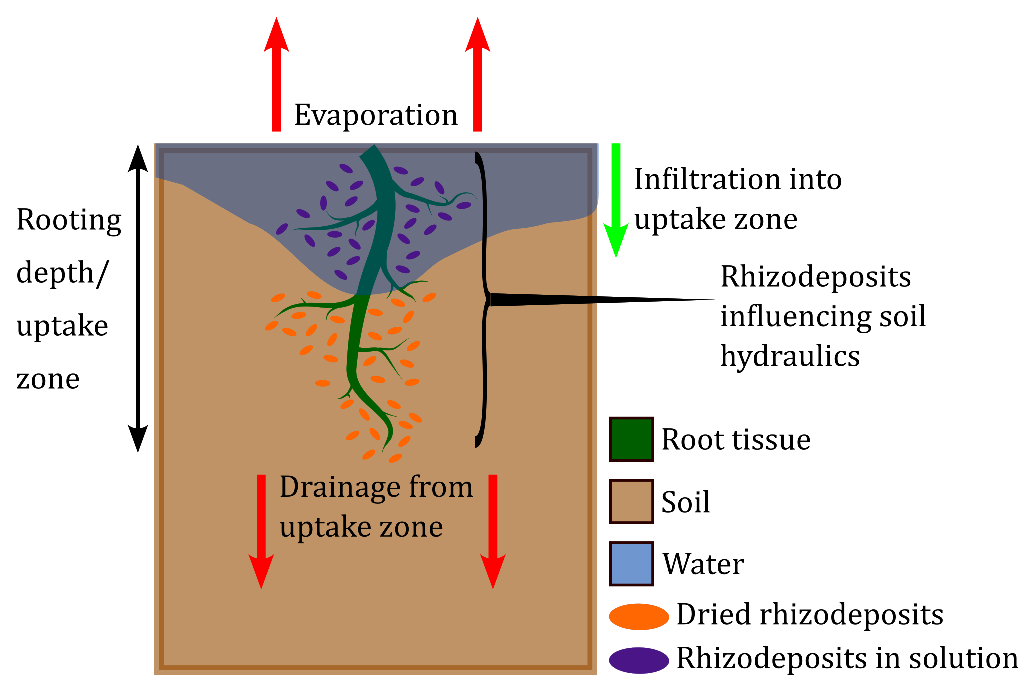
\includegraphics[width = 0.75\linewidth, keepaspectratio]{concept_figure_10_10_24.eps}
	\caption{Rhizodeposits and root water uptake. The uptake performance of a plant is affected by the availability of water within the rooted regions of the soil. This figure shows the various processes that determine levels of water availability, all of which are influenced by the presence of rhizodeposits.}
	\label{figure: processes}
\end{figure}

\section{Materials and Methods}
\subsection{A coupled model for soil water and rhizodeposit dynamics}\label{subsec: models}  
Assuming a soil domain with depth~$L$ and spatial variable~$x$, and a temporal interval with final time~$T>0$, the relationship between soil hydraulics, root rhizodeposits, and root water uptake is modelled by a system of equations that couples a modified Richards equation~\citep{richards1931capillary} solved for soil water pressure head~$h$~$[\text{L}]$:
\begin{linenomath*}
	\begin{equation}\label{model: water transport}
		\begin{aligned}
			\partial_t\theta(h) + \partial_x\mathbf{q} &= - S &x\in(-L,0),~t\in(0, T],\\
			\mathbf{q} &= g_0 &x = 0,~t\in(0, T],\\  
			-\mathbf{q} &= g_L &x = -L,~t\in(0, T],\\
			h &= h_0 & x\in(-L,0),~t=0, 
		\end{aligned}
	\end{equation}
\end{linenomath*}	
with an advection diffusion equation solved for rhizodeposit concentration in solution~$c_w$~$[\text{ML}^{-3}]$:
\begin{linenomath*}
	\begin{equation}\label{model: rhizodeposits in solution}
		\begin{aligned}
			\partial_t{(\theta(h) c_w)} - \partial_x(\theta(h) D_w\partial_xc_w - \mathbf{q}c_w) &= \rho\kappa_wc_d - \theta(h)\kappa_dc_w + f  
			&x\in(-L,0),~t\in(0, T],\\
			 - (\theta(h) D_w\partial_xc_w - \mathbf{q}c_w)&= 0 &x = 0,~t\in(0, T],\\
			 \theta(h) D_w\partial_xc_w - \mathbf{q}c_w&= 0 &x = -L,~t\in(0, T],\\  
			 c_w & = c_{w,0} &x\in(-L,0),~t=0,	 
		\end{aligned}
	\end{equation}
\end{linenomath*}
and an ordinary differential equation solved for the concentration of rhizodeposit dried to the soil surface~$c_d$~$[\text{MM}^{-1}]$:  
\begin{linenomath*}
	\begin{equation}\label{model: dried rhizodeposits}
		\begin{aligned}
			\rho\partial_tc_d &= \theta(h)\kappa_dc_w - \rho\kappa_wc_d &x\in(-L,0),~t\in(0, T],\\
			c_d & = c_{d, 0} &x\in(-L,0),~t=0.
		\end{aligned}
	\end{equation}
\end{linenomath*}
In~\eqref{model: water transport}, soil water content is given by~$\theta$~$[\text{L}^3\text{L}^{-3}]$, root water uptake by~$S$~$[\text{T}^{-1}]$, and the flux conditions at the upper surface and base of the soil by~$g_0$ and $g_L$ respectively. The movement of water through the soil is driven by the Darcy-Buckingham flux~\citep{darcy1856fontaines}
\begin{linenomath*}
	\begin{equation}\label{model: water flux}
		\begin{aligned}
			\mathbf{q} = - K(h; c_w, c_d)\partial_x(h + x),
		\end{aligned}
	\end{equation}
\end{linenomath*}
with~$K$~$[\text{LT}^{-1}]$ being the hydraulic conductivity, and~$\mathbf{q}$ appears as the advective term in the flux of root rhizodeposits in solution. The remaining terms in~\eqref{model: rhizodeposits in solution} and~\eqref{model: dried rhizodeposits} are the rhizodeposit diffusion coefficient~$D_w$~$[\text{L}^2\text{T}^{-1}]$, the soil bulk density~$\rho$~$[\text{ML}^{-3}]$, a source term~$f$~$[\text{ML}^{-3}\text{T}^{-1}]$ for the release of rhizodeposits into the soil solution by the plant roots, and the rates at which dried rhizodeposits join the soil solution~$\kappa_w$~$[\text{T}^{-1}]$ and rhizodeposits in solution dry to the soil surface~$\kappa_d$~$[\text{T}^{-1}]$.
 
The influence of rhizodeposits is incorporated into the water transport and uptake model~\eqref{model: water transport} through modifications to the \cite{van1980closed} and \cite{mualem1976new} formulations of the functions for water content and hydraulic conductivity:
\begin{linenomath*}
	\begin{equation}\label{model: water retention}
		\begin{aligned}
			\theta(h; c_w, c_d) = \theta_r + (\theta_s-\theta_r)S_e(h; c_w, c_d),\\
		\end{aligned}
	\end{equation}
	\begin{equation}\label{model: hydraulic conductivity}
		\begin{aligned}
			\qquad \quad K(h; c_w, c_d) = K^* + \alpha_KK_s(c_w, c_d)K_r(h; c_w, c_d),
		\end{aligned}	
	\end{equation}		
\end{linenomath*}
where the effective soil saturation~$S_e$ in~\eqref{model: water retention}, the saturated hydraulic conductivity~$K_s$~$[\text{LT}^{-1}]$, and the effective hydraulic conductivity~$K_r$ in~\eqref{model: hydraulic conductivity} are functions of rhizodeposit concentration. The terms $\theta_r$ and~$\theta_s$ in~\eqref{model: water retention} give the residual and saturated soil water contents respectively and parameters~$K^*$~$[\text{LT}^{-1}]$ and~$\alpha_K$ are included in~\eqref{model: hydraulic conductivity} to account for the fact that 
water content and hydraulic conductivity values at a given pressure head are generally lower if a soil is wetting than if it is drying. This hysteresis exists because the processes that occur when a soil drains are generally governed by the activity in the smaller pores whereas soil wetting tends to involve the larger pores more. Also, the contact angles between the menisci and the soil surface are different depending on whether water is entering or draining from a pore~\citep{van2011hydraulic, zhou2013contact}. In~\eqref{model: water retention} the phenomenon of hysteresis is incorporated by the effective saturation
\begin{linenomath*}
	\begin{equation}\label{model: effective saturation}
		\begin{aligned}
			S_e(h;c_w, c_d)=\frac{1}{(1+|\alpha(c_w, c_d) h|^{n})^{m}}.
		\end{aligned}
	\end{equation}  
\end{linenomath*}
Here~$n$ and~$m=1-\frac{1}{n}$ are shape parameters and the parameter~$\alpha$~$[L^{-1}]$, relating to inverse pore air entry pressure, takes different values depending on whether the soil is wetting or drying such that
\begin{linenomath*}
	\begin{equation}\label{model: inverse air entry pressure head}
		\begin{aligned}
			\alpha(c_w, c_d) =
			\begin{cases}
				\alpha^w(c_w, c_d) &\text{if wetting,}\\
				\alpha^d(c_w, c_d) &\text{if drying,}
			\end{cases}
		\end{aligned}
	\end{equation}
\end{linenomath*}
with~$\alpha^w \geq \alpha^d$~\citep{kool1987development}. Therefore, if at a given pressure head~$h_\Delta$ and  water content~$\theta_\Delta$ there is a switch from drying to wetting or vice versa, then the value of~$\alpha$ will also switch. To maintain the continuity of~$\theta$ when this happens, the residual and saturated water contents also switch between different values for wetting and drying:
\begin{linenomath*}
	\begin{equation}\label{model: hysteretic residual and saturated}
		\begin{aligned}
			\theta_{r}= 
			\begin{cases}
				\frac{(\theta_\Delta - \theta_{s,0}S_e(h_\Delta))}{1- S_e(h_\Delta)} &\text{if }\alpha=\alpha^w,\\
				\theta_{r,0} &\text{if }\alpha=\alpha^d, 
			\end{cases}\qquad
			\theta_{s} =
			\begin{cases}
				\theta_{s,0} &\text{if }\alpha=\alpha^w,\\
				\frac{\theta_\Delta - \theta_{r,0}(1-S_e(h_\Delta))}{S_e(h_\Delta)}&\text{if }\alpha =\alpha^d.
			\end{cases}			
		\end{aligned}
	\end{equation}
\end{linenomath*}   
This affects the value 
of~$K$ through the effective hydraulic conductivity~\citep{mualem1976new, van1980closed}:
\begin{linenomath*}
	\begin{equation}\label{model: relative conductivity}
		\begin{aligned}
			K_r(h; c_w, c_d)
			=&
			\Bigg(\frac{2(\theta_{s, 0} - \theta_{r,0})S_e(h_\Delta; c_w, c_d) + \varepsilon\big(1-2S_e(h_\Delta; c_w, c_d)\big)}{2(\theta_{s,0} - \theta_{r,0})}\Bigg)^l\\
			&\cdot
			\Bigg(1 - \Bigg(1 - \Bigg(\frac{2(\theta_{s,0} - \theta_{r,0})S_e(h_\Delta; c_w, c_d) + \varepsilon\big(1-2S_e(h_\Delta; c_w, c_d)\big)}{2(\theta_{s,0} - \theta_{r,0})}\Bigg)^\frac{1}{m}\Bigg)^{m}\Bigg)^2,
		\end{aligned}
	\end{equation}
\end{linenomath*}
where the parameter~$l$ denotes the tortuosity of the porous structure. Moreover, hysteresis is also incorporated into~$K$ through a saturated hydraulic conductivity term that switches between values for wetting and drying soil~\citep{vogel1996hydrus}:
\begin{linenomath*}
	\begin{equation}\label{model: saturated hydraulic conductivity}
		\begin{aligned}
			K_{s}(c_w, c_d) =
			\begin{cases}
				K_s^w(c_w, c_d) &\text{if wetting,}\\
				K_s^d(c_w, c_d) &\text{if drying,}
			\end{cases}
		\end{aligned}
	\end{equation}
\end{linenomath*}
with~$K_s^d>K_s^w$. Like in~\eqref{model: hysteretic residual and saturated}, the parameters~$K^*$ and~$\alpha_K$ in~\eqref{model: hydraulic conductivity} are also formulated so as to maintain the continuity of~$K$ if a switch between wetting and drying occurs at~$(h_\Delta,\theta_\Delta, K_\Delta)$~\citep{vogel1996hydrus}:
\begin{linenomath*}
	\begin{equation}\label{model: hydraulic conductivity hysteresis parameters}
		\begin{aligned}
			K^*&= 
			\begin{cases}
				K_s^wK_r(0)\Big(1-\frac{K_\Delta - K_s^wK_r(0)}{K_s^wK_r(h_\Delta) - K_s^wK_r(0)}\Big) \ &\text{if }K_s = K_s^w,\\
				 0 &\text{if }K_s = K_s^d,
			\end{cases}\\
			\alpha_K
			&=
			\begin{cases}
				\frac{K_\Delta-K_s^wK_r(0)}{K_s^wK_r(h_\Delta) - K_s^wK_r(0)} \qquad\qquad\qquad\qquad\ \ \text{if }K_s = K_s^w,\\
				\frac{K_\Delta}{K_s^dK_r(h_\Delta)} \qquad\qquad\qquad\qquad\qquad\qquad\quad \text{if }K_s = K_s^d.
			\end{cases} 			
		\end{aligned}
	\end{equation}
\end{linenomath*}   

The surface tension of soil water~$\gamma$ and the contact angle~$\vartheta$ of its menisci with pore surfaces have been shown to vary considerably according to the concentration of rhizodeposits and the species of plant from which these were released~\citep{ahmed2016drying, naveed2018rhizosphere, naveed2019surface}. This study will focus on wheat plants and in this case there is evidence that rhizodeposits increase the soil-water contact angle~\citep{zickenrott2016efficient}, and decrease the surface tension of the soil solution~\citep{read2003plant}. To account for this within~$\theta$, the approach of~\cite{karagunduz2001influence} is employed and scaling factors are introduced into $\alpha$, such that for~$(c_w,c_d)\in[0,\infty)^2$, 
\begin{linenomath*}
	\begin{equation}\label{model: alpha vs rhizodeposits}
		\begin{aligned}
			\alpha^w(c_w,c_d) = \frac{\gamma(c_w)\cos(\vartheta_0)}{\gamma_0\cos(\vartheta(c_d))}\alpha_0^w,
		\end{aligned}
		\quad
		\text{and}
		\quad
		\begin{aligned}
			\alpha^d(c_w) = 
			\frac{\gamma_0}{\gamma(c_w)}\alpha_0^d,			 
		\end{aligned}
	\end{equation}
\end{linenomath*}
where~$\gamma_0$ and~$\vartheta_0$ are the surface tension and contact angle values in the absence of rhizodeposits, and~$\alpha_0^w$ and~$\alpha_0^d$ are the corresponding wetting and drying values of~$\alpha$. In the formulations of~\eqref{model: alpha vs rhizodeposits} a rhizodeposit-induced reduction in surface tension will decrease~$\alpha^w$ and increase~$\alpha^d$, which means the associated pressure head to a given water content will be decreased in wetting soil and increased in drying soil. It is also assumed that in soil draining from a wet state the majority of rhizodeposits will be in solution and, hence, the terms in~\eqref{model: alpha vs rhizodeposits} are formulated so that soil-water contact angle will only have an effect during the wetting of the soil. Here an increase in contact angle will mean that the pressure head associated to a given water content during wetting is increased. In a similar way, to incorporate into~$K$ the effect of rhizodeposit-induced decreases in surface tension and increases in soil-water contact angle, the saturated hydraulic conductivities are formulated so that, for~$(c_w,c_d)\in[0,\infty)^2$,
\begin{linenomath*}
	\begin{equation}\label{model: Ks vs rhizodeposits}
		\begin{aligned}
			K_s^z(c_w,c_d) = K_{s,0}^z\cdot\Big(\frac{\gamma_0}{\gamma(c_w)}\Big)^\beta\frac{\cos(\vartheta(c_d))}{\cos(\vartheta_0)},
		\end{aligned}
	\end{equation}
\end{linenomath*}
where~$z=w,d$. This formulation of saturated hydraulic conductivity~\eqref{model: Ks vs rhizodeposits}, was informed by the work of~\cite{gomez2025exudates} where it was found that winter wheat exudates in solution facilitated the wetting of a transparent soil composed of Nafion$^{\text{TM}}$ particles. Moreover, this facilitation outweighed the soil hydrophobicity caused by some of the same exudates being dried onto the particles prior to the experiment. Assuming that rhizodeposit-induced reductions in liquid surface tension  and increases to soil-water contact angle were what caused the facilitation to wetting and soil hydrophobicity respectivley, the exponent~$\beta$ in~\eqref{model: Ks vs rhizodeposits} determines the extent to which the effects of reduced-surface tension dominate over increased contact angle. Thus, leading to improved hydraulic conductivity and facilitated water infiltration.

As in~\citep{vsimuunek2009modeling}, root water uptake in~\eqref{model: water transport} is modelled with a macroscopic sink term~$S$ incorporating water availability, root distribution, and potential plant transpiration~$\mathcal{T}_\text{p}$~$[LT^{-1}]$:
\begin{linenomath*}
	\begin{equation}\label{model: root water uptake}
		\begin{aligned}
			S(x, h) = \alpha_f(h)NRLD(x)\mathcal{T}_\text{p}\frac{1}{\max{(\omega(t),\omega_c)}}.
		\end{aligned}
	\end{equation}
\end{linenomath*}   
The dependence of uptake on the level of soil water content is included in~$S$ through the dimensionless stress response function~$0\leq\alpha_f\leq1$, and  the plant's capacity to reach the water within the soil is accounted for by the normalised root length density~$NRLD$~$[L^{-3}]$, which is a continuous function that gives the distribution of root length within the soil. The potential plant transpiration is formulated as~$\mathcal{T}_\text{p} =~\text{ET}_0\text{K}_{\text{cb}}$, where ~$\text{ET}_0$~$[\text{LT}^{-1}]$ is the reference evapotranspiration and~$\text{K}_{\text{cb}}$~$[-]$ is the basal crop coefficient~\citep{allen1998crop}. The measure of the global water stress experienced by the plant is given by the function
\begin{linenomath*}
	\begin{equation}\label{model: global water stress}
		\begin{aligned}
			\omega(t) = \int_\Omega\alpha_f(h(x, t))NRLD(x)dx
		\end{aligned}
	\end{equation}
\end{linenomath*}		
and the capacity of the plant to compensate for poor water availability in one soil region by increasing uptake in zones of higher saturation is reflected in the value of the critical water stress index~$\omega_c$~\citep{cai2018parameterization}. The boundary condition at the soil surface is
\begin{linenomath*}
	\begin{equation}\label{model: boundary condition soil surface}
		\begin{aligned}
			g_0(h, t) = \text{K}_e(h)\text{ET}_0 + RO(h,t) - P(t) 
		\end{aligned}
	\end{equation}
\end{linenomath*}
where~$\text{K}_e$~$[-]$ is a function that determines the proportion of total evapotranspiration that coming from evaporation,~$P$~$[\text{LT}^{-1}]$ the precipitation rate and~$RO$~$[\text{LT}^{-1}]$ the run-off of water that occurs when precipitation cannot enter the soil due to the surface already being fully saturated:
\begin{linenomath*}
	\begin{equation}\label{model: runoff function}
		\begin{aligned}
			RO(h,t) = P(t)\Big(1+\frac{\exp(a(\theta(h)-\theta_{s,0})) - 1}{\exp(a(\theta(h)-\theta_{s,0})) + 1}\Big). 
		\end{aligned}
	\end{equation}
\end{linenomath*}
Here the constant~$a>0$ is set to a large enough value so that if the surface is fully saturated ($\theta = \theta_{s, 0}$) then~$RO = P$. On the lower boundary~$x=-L$, the condition of free drainage is assumed, which translates as~$g_L(h) = K(h)$. The source term~$f$ in~\eqref{model: rhizodeposits in solution} for the release of rhizodeposits into the soil is formulated as follows:
\begin{linenomath*}
	\begin{equation}\label{model: rhizodeposit release}
		\begin{aligned}
			f(x,h) = \lambda\theta(h) SAD(x),
		\end{aligned}	
	\end{equation}
\end{linenomath*}
where~$\lambda$~$[\text{M}\text{L}^{-2}\text{T}^{-1}]$ is the rate at which rhizodeposits are released from the surface of the root and $SAD$~$[\text{L}^{-1}]$ is the root surface area density, a continuous function representing the distribution of root surface area throughout the soil. 

\subsection{Parametrisation and Calibration}\label{subsec: parametrisation and calibration}  	      
The functions for normalised root length density~$NRLD$ and surface area density~$SAD$ were constructed for 3 winter wheat root systems of ages 6, 15 and 30 days. These root systems were generated from CRootBox~\citep{schnepf2018crootbox} using the default settings for wheat systems and their respective architectures are shown in Figure~\ref{figure: simulated root systems}). The methods previously employed and described in~\citep{mair2022model, mair2023can} were used to convert the architecture data of each root system into density functions for the distributions of root length and surface area, which took values in the 3D soil domain whose length, breadth and depth were defined by the furthest reaching roots across each of the root systems. These functions were then averaged laterally across the 3D domain to produce~$NRLD$ and~$SAD$ as functions of 1D space~$(-L,0)$, where~$L = 53\text{cm}$ is the greatest depth reached by any root of the 3 systems. 
To explicitly model the ways in which rhizodeposits induce a reduction in soil water surface tension~$\gamma$, and an increase in the contact angle~$\vartheta$ between menisci and the soil pore surface, the data of~\cite{read2003plant} and~\cite{zickenrott2016efficient} were used to fit the following functions:
\begin{linenomath*}
	\begin{equation}\label{model: surface tension}
		\begin{aligned}
			\gamma(c_w) = 47.5 +\frac{72.9-47.5}{1 + \exp(18.79(c_w-0.36))},
		\end{aligned}
	\end{equation}
	and
	\begin{equation}\label{model: contact angle}
		\begin{aligned}
			\vartheta(c_d) = \frac{3.53}{18}\pi(1+\exp(-1879.14c_d))^{-4.39}.
		\end{aligned}
	\end{equation}
\end{linenomath*}
These functions return~$\gamma_0=\gamma(0)=72.9\text{mNm}^{-1}$ and~$\vartheta_0 = \vartheta(0) = 0.0294\text{rad}$ as the surface tension and contact angle when there are no rhizodeposits present. Explicit formulation of the precipitation function~$P$ is omitted but~Figures~\ref{figure: almeria_precip_evap_up} and~\ref{figure: Madrid_precip_evap_up} illustrate its form and how its parametrisation can be altered to impose different delivery patterns of a given total precipitation. Otherwise, for any remaining functions whose formulations and parameters have not been explicitly disclosed, the reader is directed to~\citep{mair2023can}.   

The sandy loam soil and winter wheat root systems were considered in all model simulations, and the majority of the values that were required to parametrise the models accordingly were taken from existing literature, see Table~\ref{table: model_parameters}. The parameter values that remained to be sourced were then the rate at which dried rhizodeposits join the soil water solution~$\kappa_w$, the rate at which rhizodeposits in solution dry to the pore surface~$\kappa_d$, and the parameter~$\beta$ that controls the size of the increase in saturated hydraulic conductivity brought about by a rhizodeposit-induced reduction in surface tension. The values of these 3 parameters were approximated through a dye tracing experiment~\citep{liu2024microcosm}, in which microcosms chambers were filled with 3 layers of the artificial transparent soil Nafion$^{\text{TM}}$, and microscopy was used to monitor the infiltration of dye solution through the medium. Adding extracted winter wheat exudates to the dye solution in the upper Nafion layer$^{\text{TM}}$,~\citep{gomez2025exudates} recorded the effect on infiltration, and the model system~\eqref{model: water transport}-\eqref{model: dried rhizodeposits}, along with an advection diffusion equation for dye concentration within the chamber, was employed to simulate the process. Bayesian optimisation~\citep{brochu2010tutorial} was then used to search the parameter space~$(\kappa_d,\kappa_w, \beta)$ and approximate the values that allowed the model system to best reproduce the experimental results. These values are shown in Table~\ref{table: model_parameters} and further details of this experimental setup and calibration procedure will be available upon publication of the manuscript~\citep{gomez2025exudates}.    

\subsection{Simulated scenarios}
To investigate the impact of rhizodeposits on root water uptake performance, the model system~\eqref{model: water transport},~\eqref{model: rhizodeposits in solution} and~\eqref{model: dried rhizodeposits} was separately parametrised for each age of root system. This not only entailed different functions of~$NRLD$ and~$SAD$ but also progressively larger values of basal crop coefficient~$\text{K}_{\text{cb}}$ to reflect the increase in transpiration rate with plant age. Specifically,~$\text{K}_{\text{cb}} = 0.15, 0.32, 0.5$ for the 6, 15 and 30-day old root systems respectively. For every root system parametrisation, 6 precipitation regimes were considered. In 3 of these regimes the precipitation function~$P$ was formulated to deliver a total of~$0.12\text{cm}$ rainfall over a time period of~$T=3\text{d}$, delivered in either 1, 2 or 3 rainfall events. In order to ensure total precipitation remained the same across all patterns, each time the total number of rainfall events was increased by 1 the duration of each rainfall event decreased by~$25\%$, along with a corresponding decrease in the rainfall rate. The other 3 precipitation regimes were defined in the same way, but with total rainfall set to~$0.28\text{cm}$. Figures~\ref{figure: almeria_precip_evap_up} and~\ref{figure: Madrid_precip_evap_up}~(a)-(c) provide a visual representation of the precipitation function~$P$ for the 6 different rainfall patterns. In each scenario, initial water content was set to a uniform value of~$\theta(h_0) = 0.69$ throughout the domain. In the scenarios that included rhizodeposits, the initial concentration of rhizodeposit in solution was set so that in the depths of soil occupied by roots~$c_{w,0}=2.5\text{mgcm}^{-3}$ but in the depths without roots~$c_{w,0}=0\text{mgcm}^{-3}$. Assuming an initial equilibrium between the dynamics of dried rhizodeposits and rhizodeposits in solution, initial dried rhizodeposit concentration was set so that~$c_{d, 0}=5.2\times10^{-4}\text{mgcm}^{-3}$ in domain depths with roots, and~$c_{d, 0}=0\text{mgcm}^{-3}$ in the depths without. Water infiltration simulations were then obtained for each root system and precipitation pattern combination, both with and without the incorporation of rhizodeposit influence, and results on soil water dynamics and root water uptake were recorded.    

\subsection{Computations}
Numerical solutions for pressure head, rhizodeposits in solution and dried rhizodeposits were obtained from the model system~\eqref{model: water transport},~\eqref{model: rhizodeposits in solution},~\eqref{model: dried rhizodeposits} using a conformal finite element method and an implicit Euler discretisation in time. The cells of the 1D domain discretisation were each~$0.593\text{cm}$ in length, and the time step size was~$ 0.001\text{d}$. Linearisation of the functions for water content and hydraulic conductivity in~\eqref{model: water transport} was carried out using the L-scheme of~\cite{list2016study}. The numerical method was implemented using the FEniCS library~\cite{AlnaesBlechta2015a} and the algorithms to construct $NRLD$ and $SAD$ from CRootBox architectures were run in Python 3 using the libraries NumPy and SciPy~\citep{harris2020array}. The visualisations of 1D root density profiles, water distributions and flux strength were generated from Paraview~\citep{ahrens2005paraview}. The plots in Figure~\ref{figure: simulated root systems} showing the architectures of the studied root systems were generated using MATLAB 2024b. The Bayesian optimisation algorithm used to calibrate model~\eqref{model: water transport}-\eqref{model: dried rhizodeposits}, was implemented using the scikit-optimise library in Python 3~\citep{tim_head_2018_1207017}. 

\section{Results}

\subsection{Effect of rhizodeposits on water infiltration}
In the case where total precipitation of 0.12cm was shared over 3 rainfall events, simulations showed that water infiltration was greater in all scenarios where rhizodeposits were present compared to when they were not~(Figure~\ref{figure: almeria_3_events_fluxes}). Downward water flux increased with each additional rainfall both with and without the presence of rhizodeposits. However, the enhancement of the flux in the presence of rhizodeposits became more and more pronounced with each rainfall event~(Figure~\ref{figure: almeria_3_events_fluxes}). It can be seen from Figure~\ref{figure: almeria_3_events_fluxes} that at all observed time points, and for each age of root system, this increased water infiltration in the presence of rhizodeposits lead to a higher water content at the soil depth where root length density was highest. Moreover, at no point of the simulation did this more powerful downward water flux appear to have caused much movement of water into deeper non-rooted soil layers.

In the scenario where a total precipitation of 0.28cm was delivered in one day~(Figure~\ref{figure: madrid_1_event_fluxes}), downward water flux was stronger than in the case where the delivery of a total precipitation of 0.12cm was split over 3 events~(Figure~\ref{figure: almeria_3_events_fluxes}), and this was true irrespective of rhizodeposit presence. Like with 0.12cm precipitation delivered in 3 events, though, when total precititation of 0.28cm was delivered in one day, the downward water flux was also always stronger with rhizodeposits present than without~(Figure~\ref{figure: madrid_1_event_fluxes}). Similarly, at 0.5 days, just after the single rainfall event, the increased downward flux of water had resulted in an increased water content in the depths of soil where the root length density of all root systems was highest. However, the magnitude of this downward water flux was greatest at 0.5 days and then decreased over the rest of the simulation~(Figure~\ref{figure: madrid_1_event_fluxes}). Furthermore, for the 6 and 15-day old root systems with rhizodeposits present and 0.28cm precipitation delivered in one event, the increased downward water flux with was excessive and after 1.5 and 2.5 days had resulted in considerable amounts of water being lost to depths with low or zero root length density~(Figure~\ref{figure: madrid_1_event_fluxes}). Since the root length density of the 30 day old root system was allocated more equally and to greater depths of the soil, this strengthened water flux to greater depths did not reduce water availability to the root system.    
  

\subsection{Effect of rhizodeposits on rates of soil surface evaporation and root water uptake}
For all root systems in all precipitation conditions, evaporation rates were lower, at every point of the 3 day simulation, with rhizodeposits present in the soil than without~(Figures~\ref{figure: almeria_precip_evap_up}~and~\ref{figure: Madrid_precip_evap_up}~(d)-(f)). It was also the case in the regimes of both lower (0.12cm) and higher (0.28cm) total precipitation, that following the onset of a rainfall event, the water uptake rates of all root systems in soils with rhizodeposits were, for a finite period of time at least, larger than those recorded for soils without rhizodeposits~(Figures~\ref{figure: almeria_precip_evap_up}~and~\ref{figure: Madrid_precip_evap_up}~(g)-(i)). For the 30-day old root system, which had the deepest rooting depth, this higher uptake rate in the presence of rhizodeposits was observed across all points in time, and this was true for the regimes with both lower (0.12cm) and higher (0.28cm) total rainfall and across all delivery patterns~(Figures~\ref{figure: almeria_precip_evap_up}~and~\ref{figure: Madrid_precip_evap_up}~(g)-(i)). Moreover, in all 3 delivery patterns of the regime with lower total precipitation~(0.12cm), the uptake rates of the 6 and 15-day old wheat plants, which had shallower root architectures, were higher when rhizodeposits were present than when they were not, and this was also true at all time points~(Figure~\ref{figure: almeria_precip_evap_up}). However, from Figure~\ref{figure: almeria_precip_evap_up}~(g) it can be seen that in the precipitation pattern where all 0.12cm is delivered in a single event, the difference between the increased uptake rate with rhizodeposits and the lower rate without rhizodeposits had almost closed by the end of the simulation. This, therefore, suggested that a higher uptake rate with rhizodeposits in the soil than without may not necessarily be maintained for the entire simulation under all combinations of total precipitation, delivery pattern and root system age. Indeed, under all 3 delivery patterns of 0.28cm of total precipitation the shallower 6 and 15-day old root systems initially assumed higher uptake rates with rhizodeposits in the soil than without but, eventually, the uptake rates of these root systems in soil without rhizodeposits overtook and maintained higher values until the end of the simulation~(Figure~\ref{figure: Madrid_precip_evap_up}). The timing of this overtake was earliest for the precipitation pattern in which all 0.28cm are delivered in one event. Finally, the last relevant finding regarding uptake rates was that within certain time intervals of these 3 day simulations (if not the entire simulation) the uptake rates of the 15-day old root system were higher than those of the 30-day old, and this was true for soils with or without rhizodeposits~(Figures~\ref{figure: almeria_precip_evap_up}~and~\ref{figure: Madrid_precip_evap_up}).

\subsection{Rhizodeposit effect on total uptake and the sensitivity to precipitation pattern and root system maturity}
Table~\ref{table: lower rainfall total uptake} shows that in all rainfall patterns with 0.12cm total precipitation, total water uptake of every age of root system was greater if rhizodeposits were present in the soil than if they were not. Moreover, it can be seen from Table~\ref{table: higher rainfall total uptake} that for all rainfall patterns of 0.28cm total precipitation the total uptake of the 30-day old root system was also always larger when rhizodeposits were present than when they were not. These results are expected given that, as previously mentioned for these cases, the heightened uptake rates in the presence of rhizodeposits were maintained over the entire simulation period. The more nuanced results regarding total uptake under the effect of rhizodeposits come, therefore, from the cases where uptake rates with rhizodeposits in the soil were at some stage overtaken by the uptake rates without. In the regimes with a total precipitation of 0.28cm, if it is delivered in 2 or 3 rainfall events, then the 6 and 15-day old root systems with rhizodeposits also continued to have higher total root water uptake than without rhizodeposits~(Table~\ref{table: lower rainfall total uptake}), despite the without-rhizodeposit uptake rates overtaking the with-rhizodeposit rates at later simulation times. However, when the entire 0.28cm was delivered in one event, the  uptake rates of the 6 and 15-day old root systems in soil with rhizodeposits were overtaken early enough during the simulation by the corresponding rates without soil rhizodeposits that the total uptakes of the 6 and 15-day old root systems ended up being lower when rhizodeposits are present in the soil than when they are not~(Table~\ref{table: higher rainfall total uptake}). This result can also be seen in Figure~\ref{figure: uptake_age_intensity} which shows that the percentage change in total water uptake that comes with the presence of rhizodeposits is negative in the case where root systems are less mature and 0.28cm of precipitation is delivered in one event. Considering root systems of all ages, there was in fact a general trend that the percentage positive change in total water uptake from including rhizodeposits in the soil decreased as the amount of total rainfall in the 3 day simulation was increased~(Figure~\ref{figure: uptake_age_intensity}). In addition, when fixing total rainfall and considering the pattern by which it was delivered, it is also true that the positive effect of rhizodeposits on total water uptake was reduced as the precipitation was delivered over fewer events~(Figure~\ref{figure: uptake_age_intensity}).

Regarding the increased uptake rates of the 15-day old root system compared to the 30-day old root system, which were observed during certain intervals of specific precipitation scenarios, the net effect on total uptake can also be seen in Tables~(\ref{table: lower rainfall total uptake},~\ref{table: higher rainfall total uptake}). In the end, there were only 4 scenarios where the 15-day old root system had greater total uptake than the 30 day old root system. Namely, when total precipitation was 0.12cm and all delivered in a single event with no rhizodeposits in the soil, when total precipitation was 0.12cm and delivered over 2 events with rhizodeposits in the soil, and for all scenarios with 0.28cm total precipitation and no rhizodeposits in the soil. 

\begin{figure}
	\centering
	\begin{subfigure}{0.275\textwidth}
		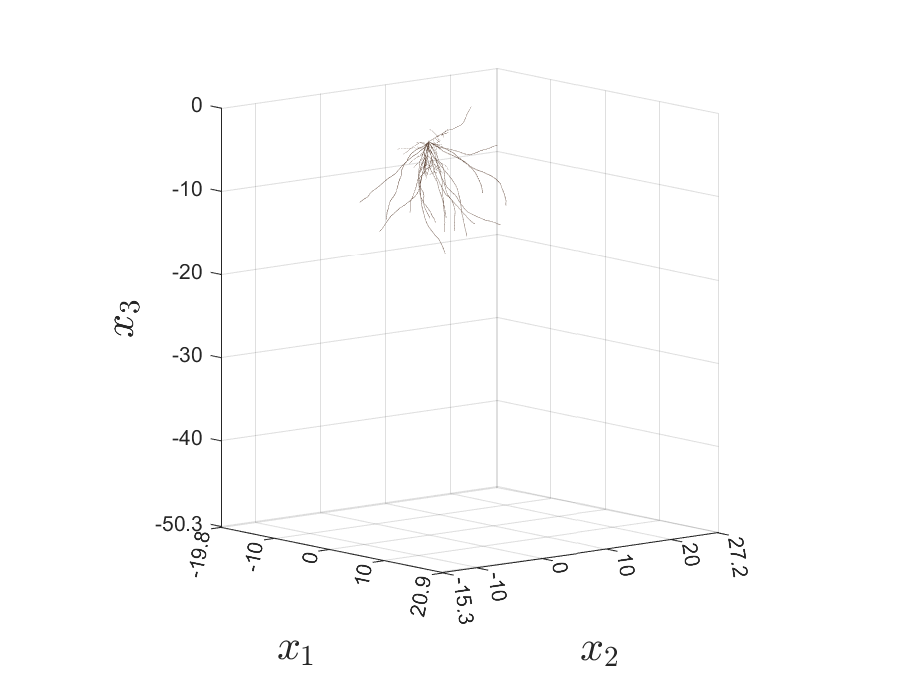
\includegraphics[width = \linewidth, keepaspectratio] {trigo6days1_3D_plot.eps}
		\caption{}
	\end{subfigure}\qquad
	\begin{subfigure}{0.275\textwidth}
		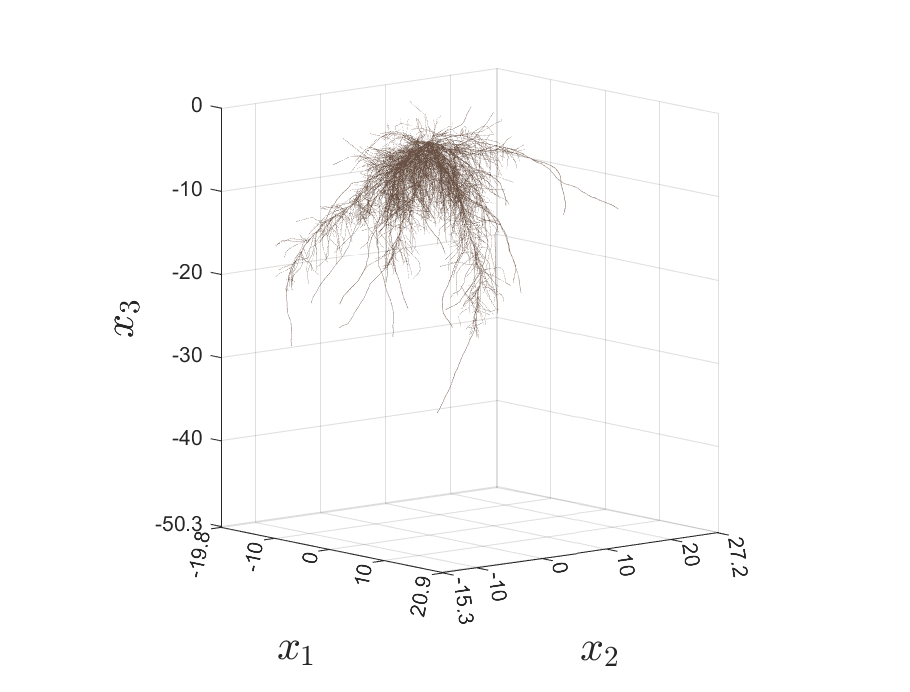
\includegraphics[width = \linewidth, keepaspectratio] {trigo15days1_3D_plot.eps}
		\caption{}
	\end{subfigure}\qquad
	\begin{subfigure}{0.275\textwidth}
		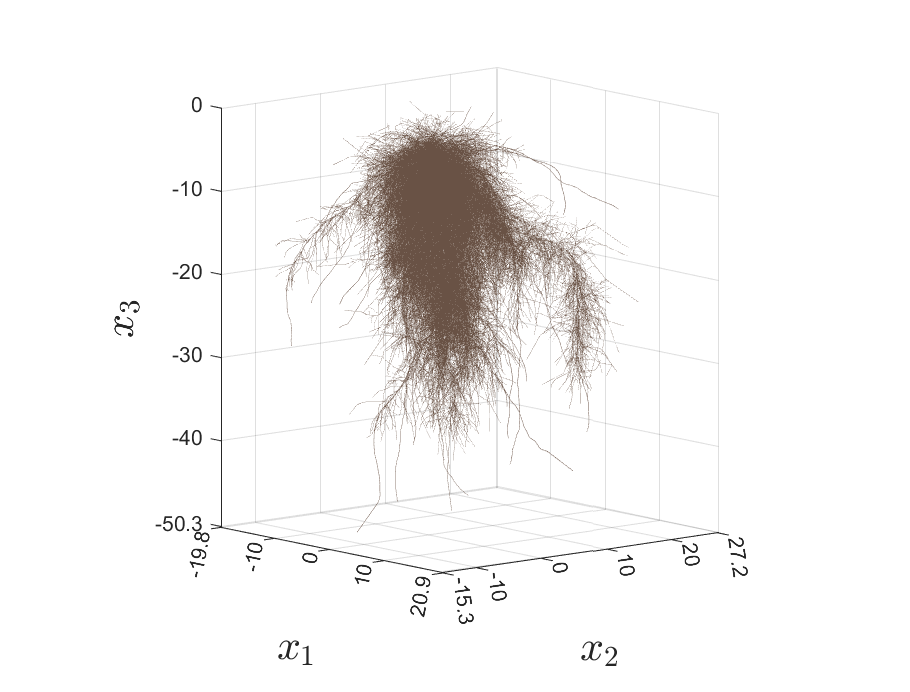
\includegraphics[width = \linewidth, keepaspectratio] {trigo30days1_3D_plot.eps}
		\caption{}
	\end{subfigure}
	\caption{Winter wheat root systems used for testing the impact of root rhizodeposits on soil water dynamics and root water uptake.~(a) 6-day old root system.~(b) 15-day old root system.~(c) 30-day old root system.}
	\label{figure: simulated root systems}
\end{figure}

\begin{figure}
	\centering
	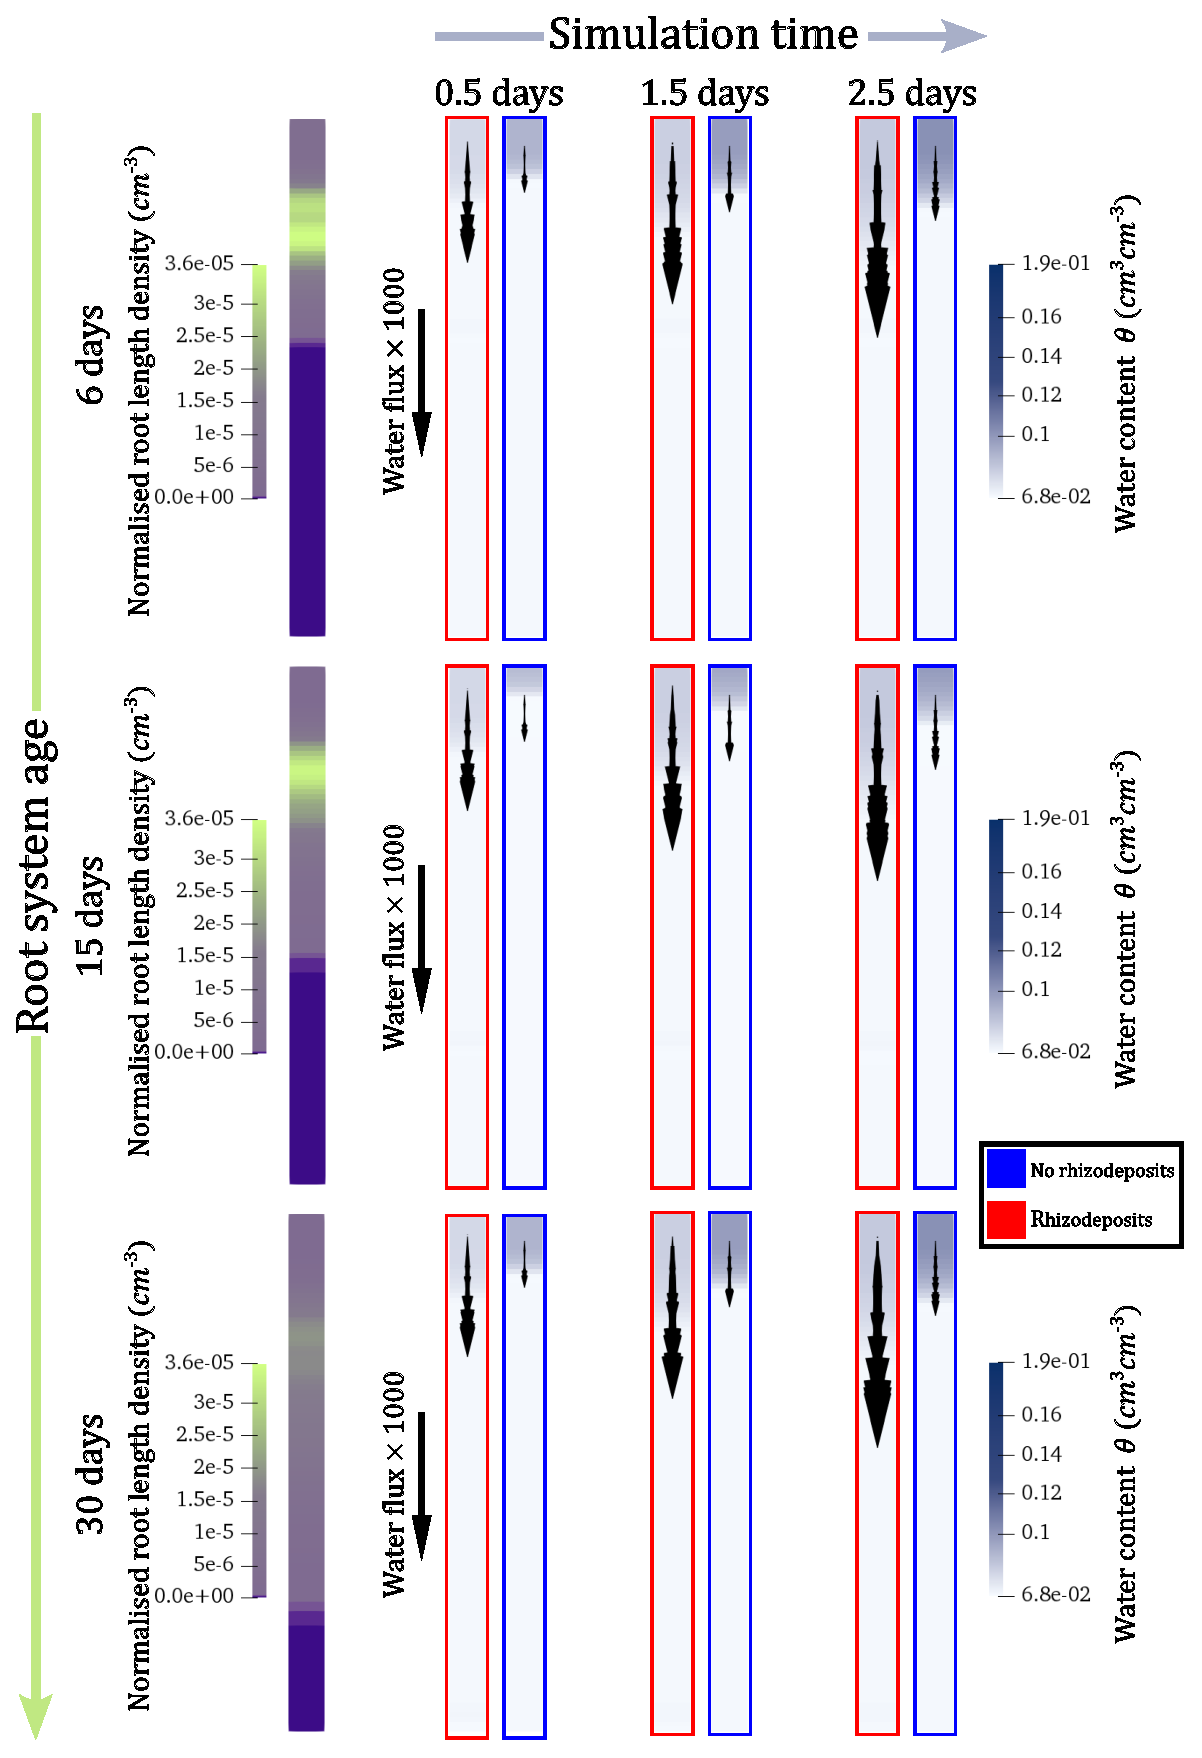
\includegraphics[width = 0.75\linewidth, keepaspectratio]{almeria_3_events.eps}
	\caption{The influence of rhizodeposits on the evolution of soil water content and flux over time under the 3-event pattern of the lower total rainfall regime. The figures of the leftmost column show the normalised root length density profiles of each plant within the 1D soil domain (age increasing downwards). The remaining columns show snapshots of the water dynamics, within this same domain, at different time points of the simulation. Each row relates to soil vegetated by the roots of each age of plant, and the arrows illustrate the strength of the flow at each time point.}
	\label{figure: almeria_3_events_fluxes}
\end{figure}

\begin{figure}
	\centering
	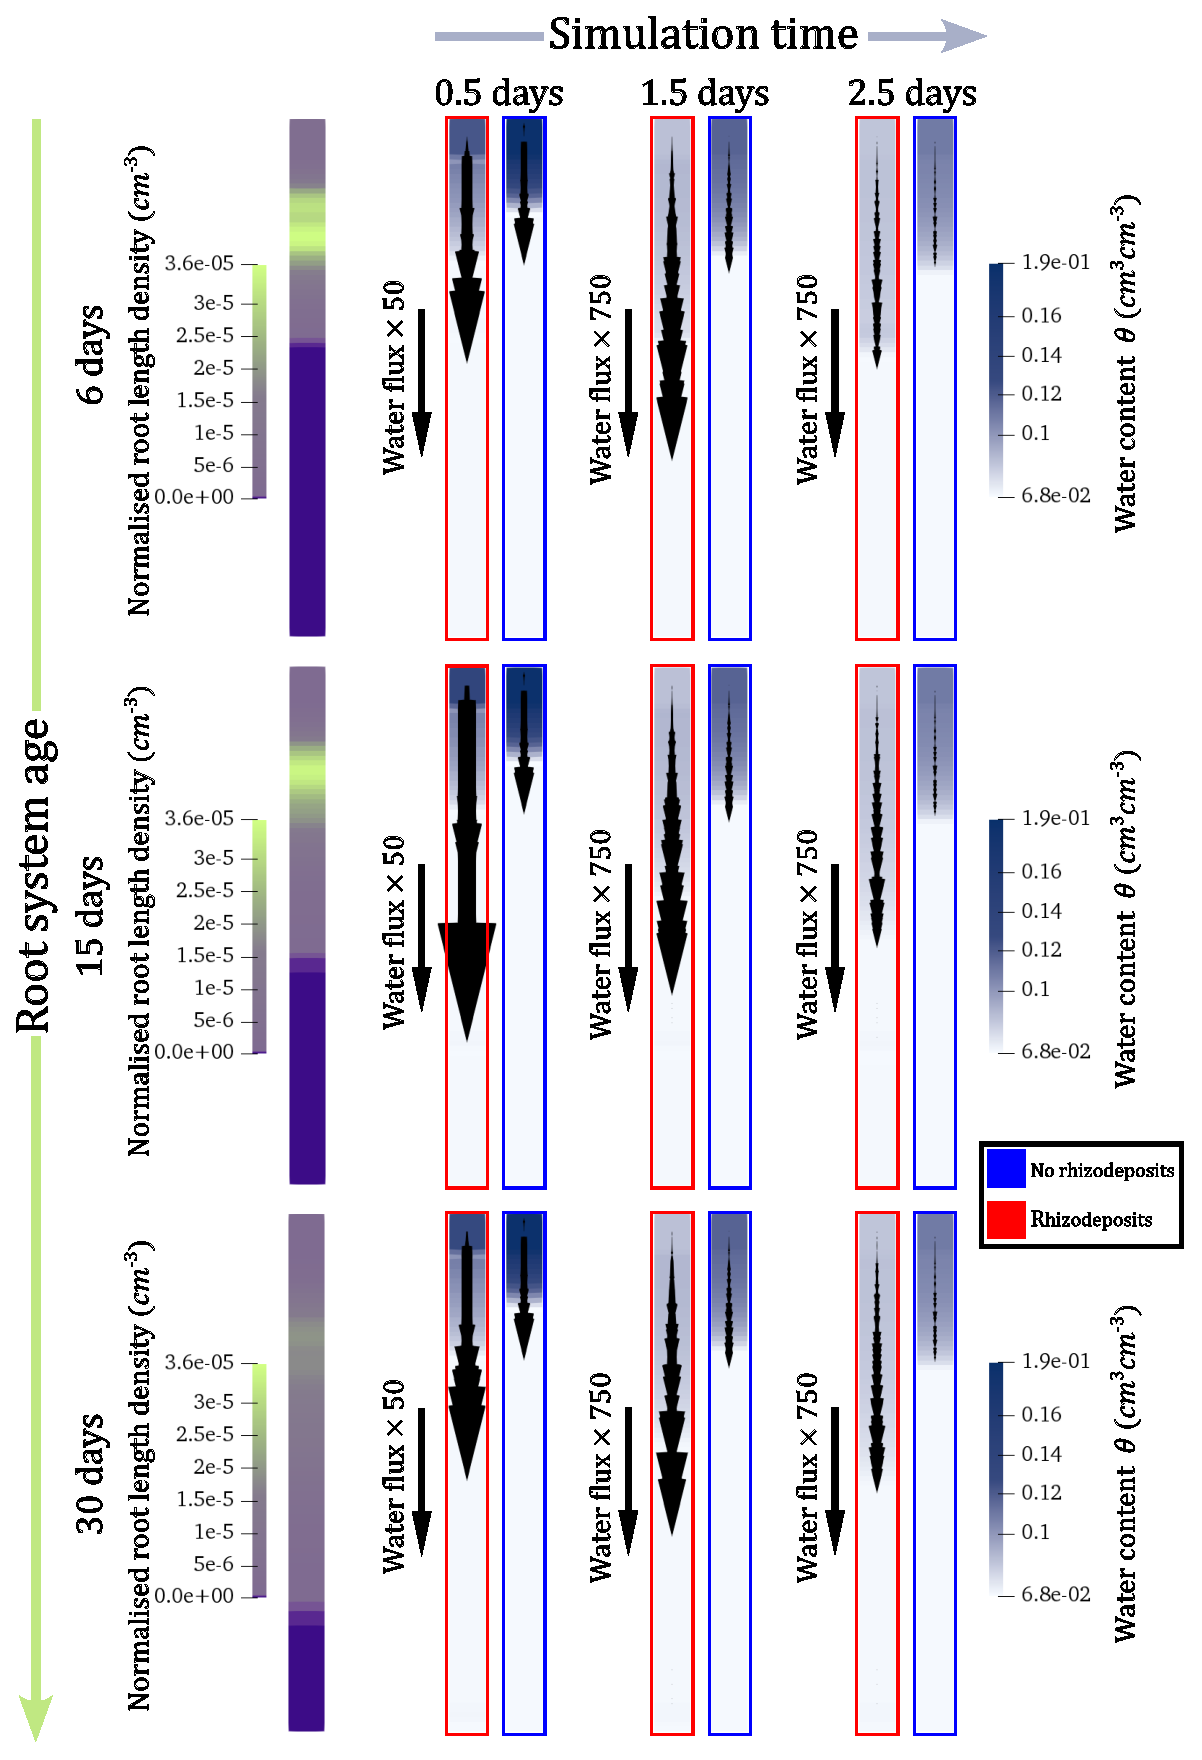
\includegraphics[width = 0.75\linewidth, keepaspectratio]{madrid_1_event.eps}
	\caption{The influence of rhizodeposits on the evolution of soil water content and flux over time under the 1-event pattern of the high-rainfall regime. The figures of the leftmost column show the normalised root length density profiles of each plant within the 1D soil domain (age increasing downwards). The remaining columns show snapshots of the water dynamics, within this same domain, at different time points of the simulation. Each row relates to soil vegetated by the roots of each age of plant, and the arrows illustrate the strength of the flow at each time point.}
	\label{figure: madrid_1_event_fluxes}
\end{figure}
  
\begin{figure}
	\centering
	\begin{subfigure}{0.32\textwidth}
		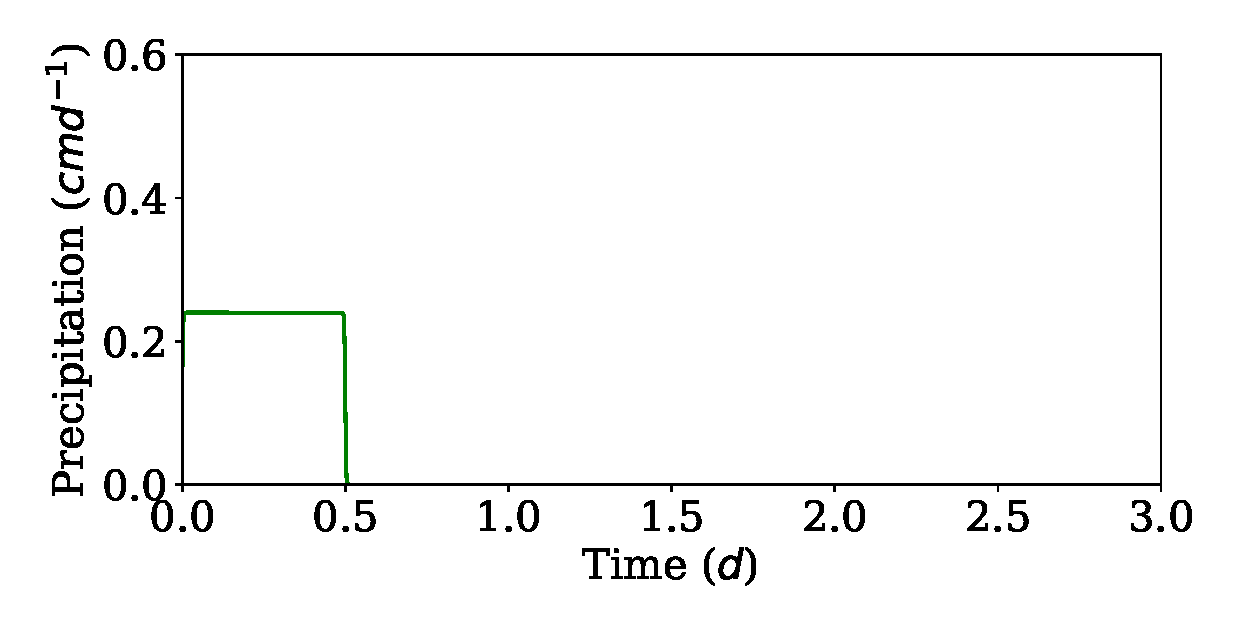
\includegraphics[width = \linewidth, keepaspectratio] {pr_ppat1ptot0_12.eps}
		\caption{}
	\end{subfigure}
	\begin{subfigure}{0.32\textwidth}
		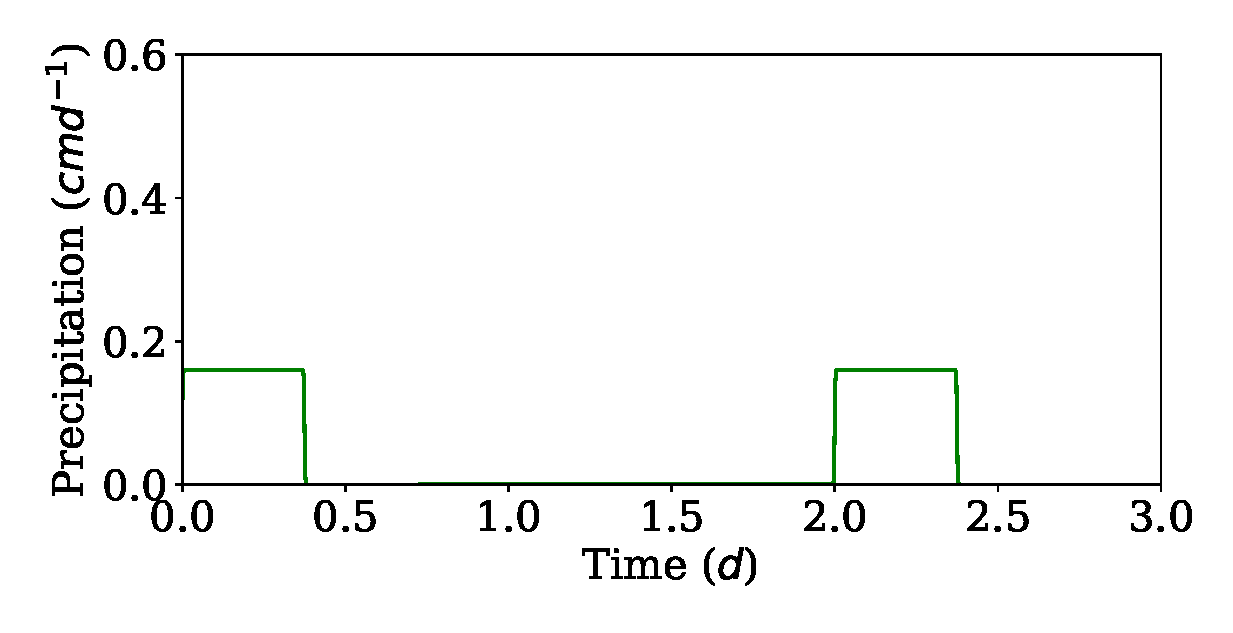
\includegraphics[width = \linewidth, keepaspectratio] {pr_ppat2ptot0_12.eps}
		\caption{}
	\end{subfigure}
	\begin{subfigure}{0.32\textwidth}
		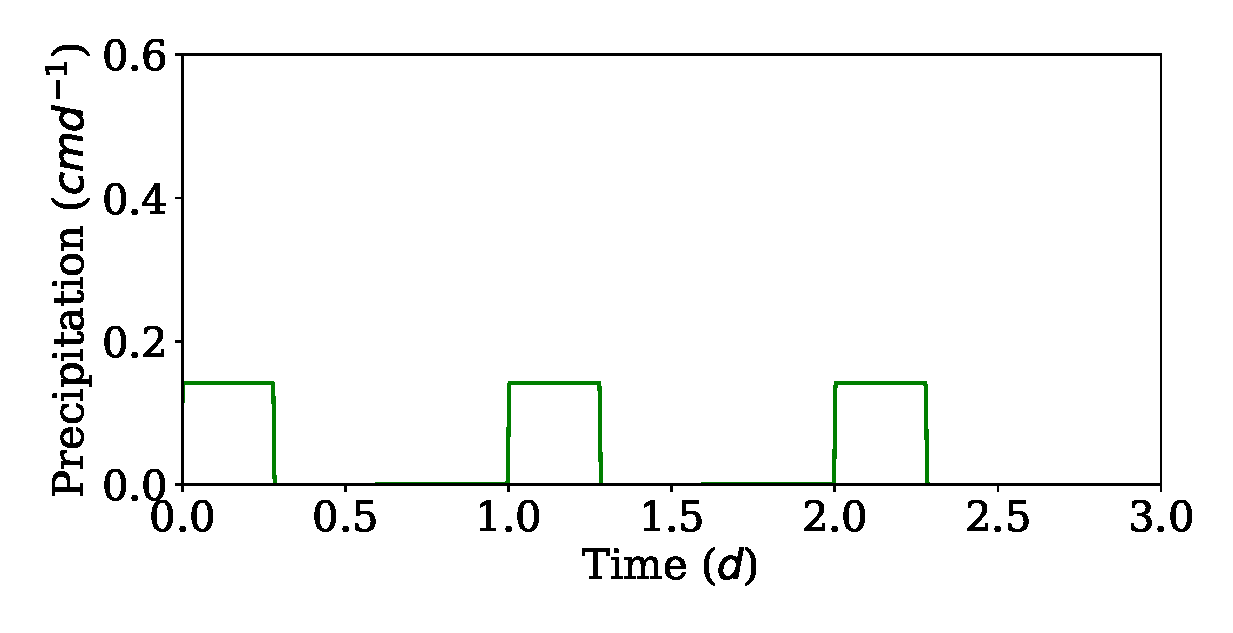
\includegraphics[width = \linewidth, keepaspectratio] {pr_ppat3ptot0_12.eps}
		\caption{}
	\end{subfigure}\\
	\begin{subfigure}{0.32\textwidth}
		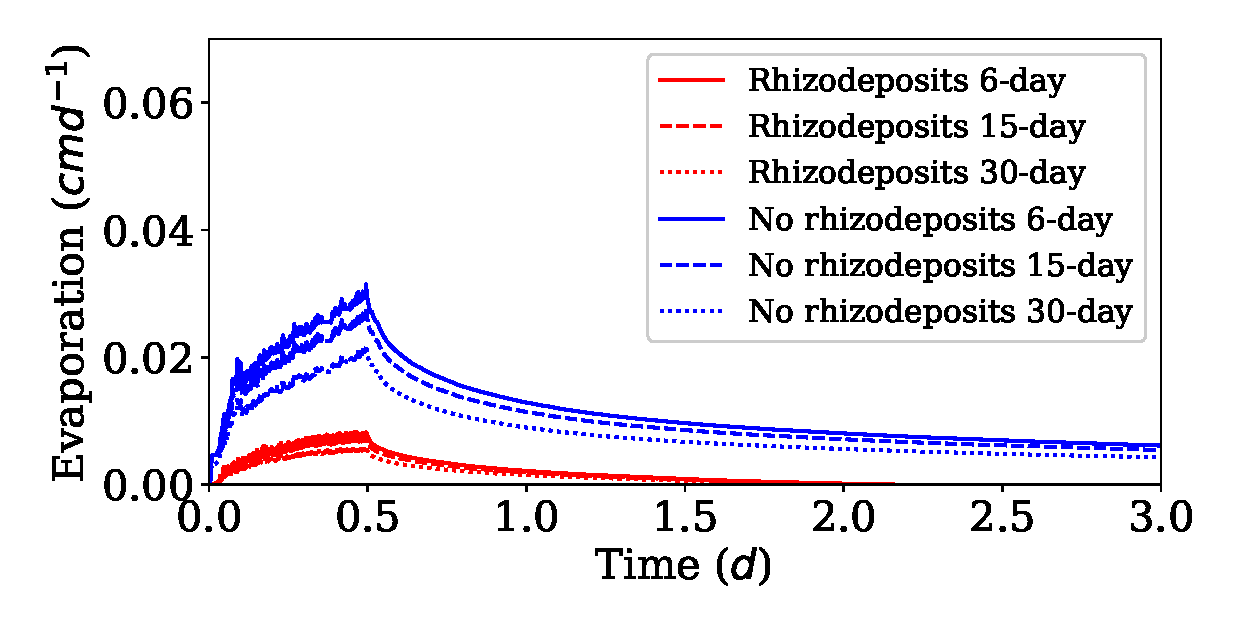
\includegraphics[width = \linewidth, keepaspectratio] {ev_ppat1ptot0_12.eps}
		\caption{}
	\end{subfigure}
	\begin{subfigure}{0.32\textwidth}
		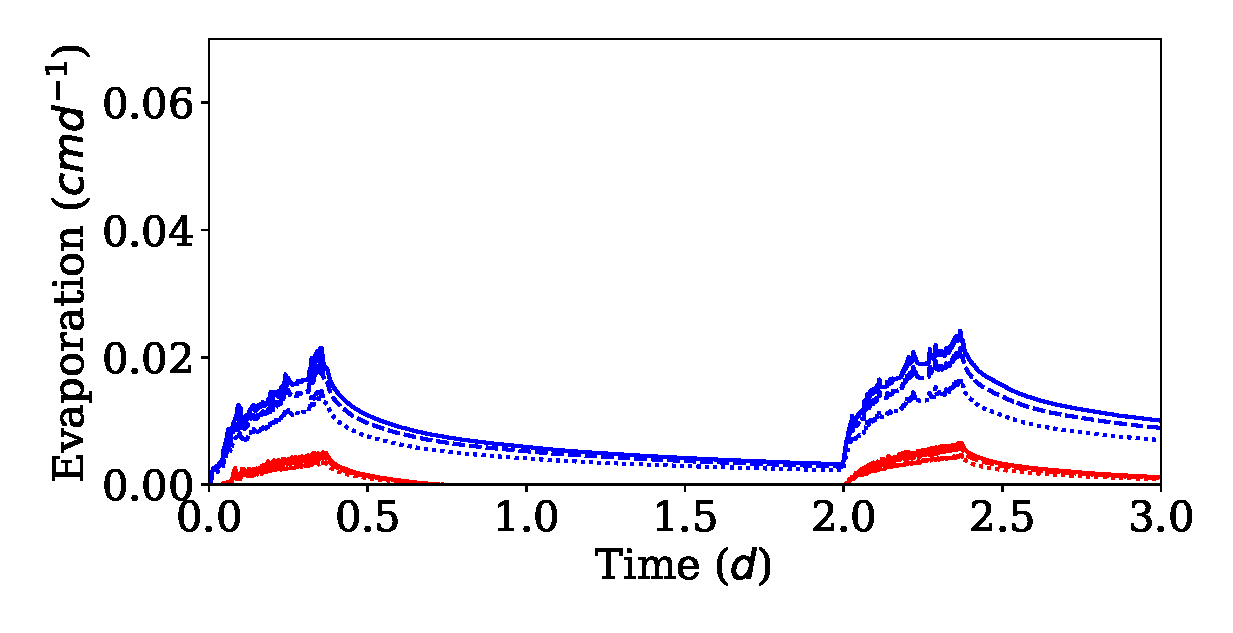
\includegraphics[width = \linewidth, keepaspectratio] {ev_ppat2ptot0_12.eps}
		\caption{}
	\end{subfigure}
	\begin{subfigure}{0.32\textwidth}
		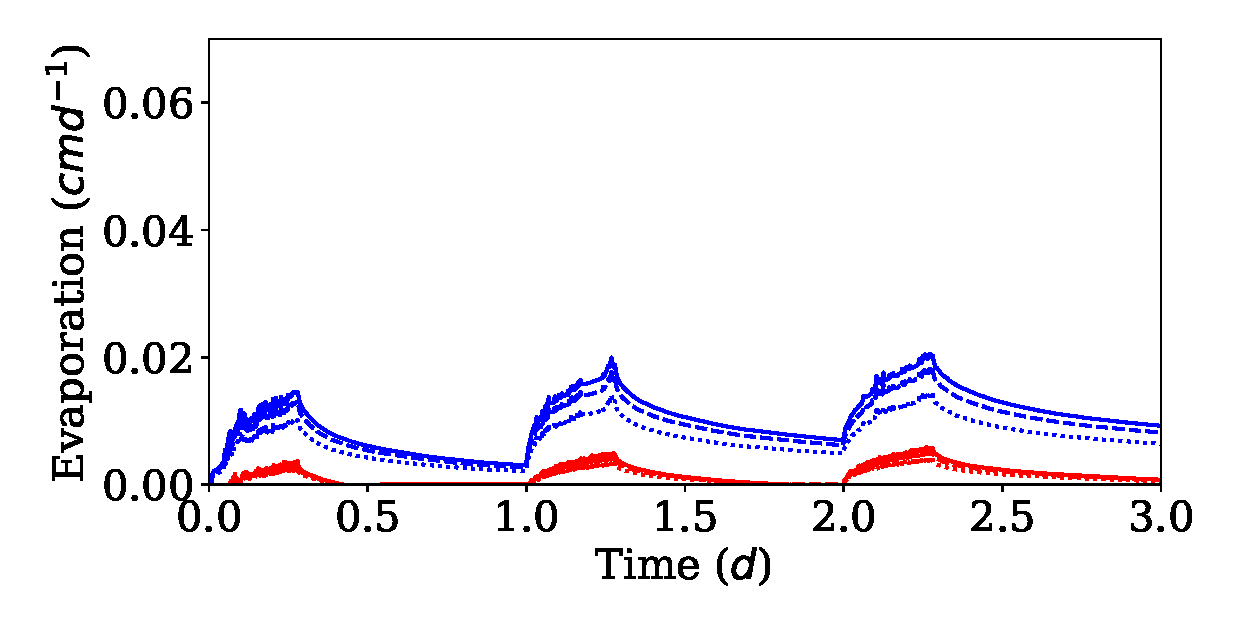
\includegraphics[width = \linewidth, keepaspectratio] {ev_ppat3ptot0_12.eps}
		\caption{}
	\end{subfigure}\\
	\begin{subfigure}{0.32\textwidth}
		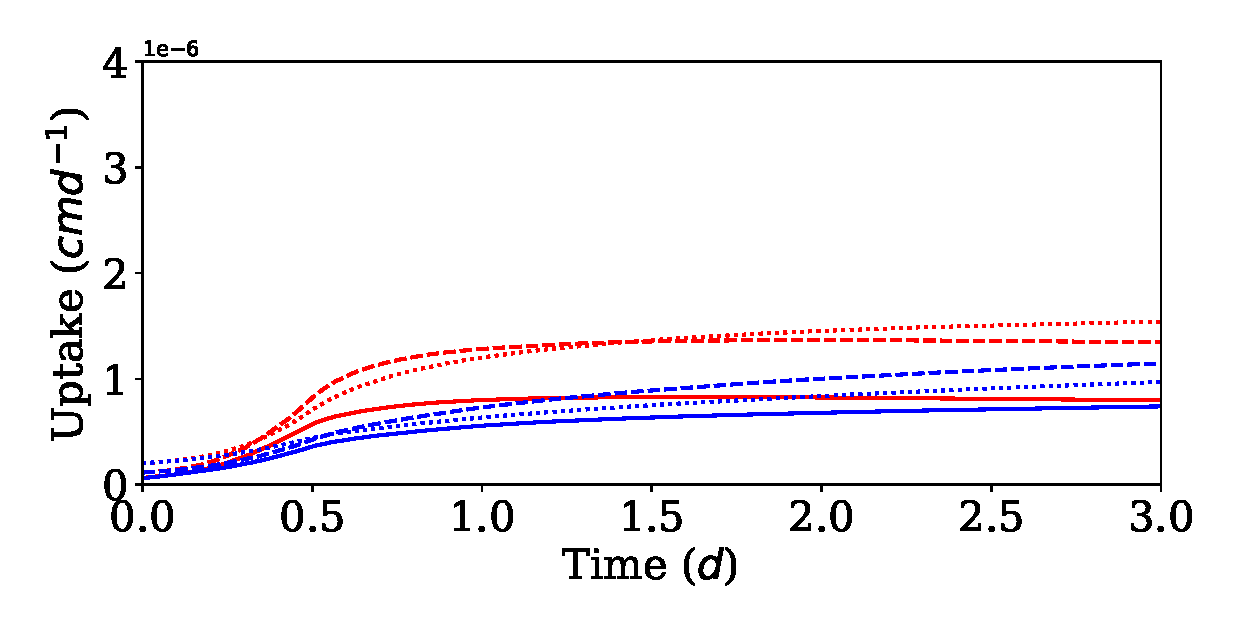
\includegraphics[width = \linewidth, keepaspectratio] {up_ppat1ptot0_12.eps}
		\caption{}
	\end{subfigure}
	\begin{subfigure}{0.32\textwidth}
		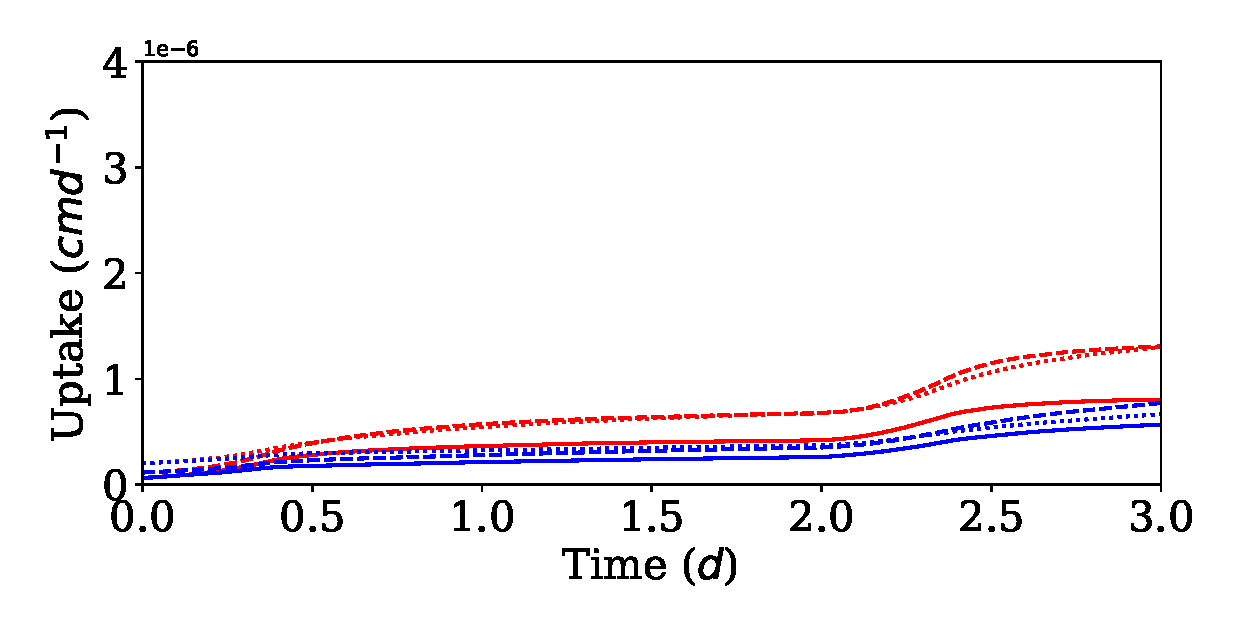
\includegraphics[width = \linewidth, keepaspectratio] {up_ppat2ptot0_12.eps}
		\caption{}
	\end{subfigure}
	\begin{subfigure}{0.32\textwidth}
		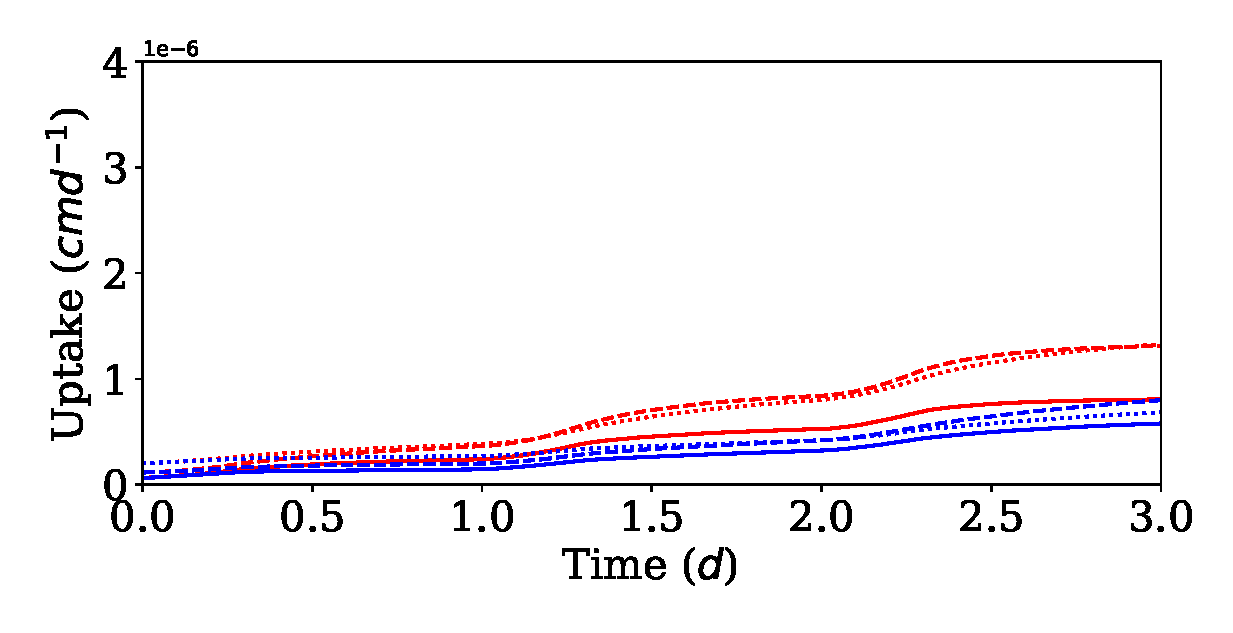
\includegraphics[width = \linewidth, keepaspectratio] {up_ppat3ptot0_12.eps}
		\caption{}
	\end{subfigure}
	\caption{The influence of rhizodeposits on root water uptake under different precipitation regimes of a lower-rainfall environment. Plots (a)-(c) show the precipitation patterns considered. The plots (d)-(f) lying directly below show the evaporation rates corresponding to each pattern and for soils occupied by each age of root system with or without rhizodeposits present. Similarly plots (g)-(i) show the corresponding uptake rates of each root system, with and without rhizodeposits present}
	\label{figure: almeria_precip_evap_up}
\end{figure}

\begin{table}
	\centering
	\smaller
	\begin{tabular}{{ |p{3cm}||p{1.55cm}|p{1.55cm}|p{1.55cm}|p{1.55cm}|p{1.55cm}|p{1.55cm}||}}
		\hline
		\multicolumn{1}{|l||}{Total rainfall} &
		\multicolumn{6}{|c||}{0.12cm}\\
		\hline
		\multicolumn{1}{|l||}{Rainfall distribution} &
		\multicolumn{2}{|c|}{1 event} &
		\multicolumn{2}{|c|}{2 events} &
		\multicolumn{2}{|c||}{3 events}\\
		\hline
		Rhizodeposits & No & Yes & No & Yes & No & Yes\\
		\hline
		Total uptake: 6-day old plant (cm)& $1.67\times10^{-6}$ & $2.12\times10^{-6}$ & $8.35\times10^{-7}$ & $1.31\times10^{-6}$ & $8.49\times10^{-7}$ & $1.32\times10^{-6}$\\
		\hline
		Total uptake: 15-day old plant (cm)& $2.38\times10^{-6}$ & $3.44\times10^{-6}$ & $1.10\times10^{-6}$ & $2.05\times10^{-6}$ & $1.12\times10^{-6}$ & $2.06\times10^{-6}$\\
		\hline
		Total uptake: 30-day old plant (cm)& $2.08\times10^{-6}$ & $3.55\times10^{-6}$ & $1.16\times10^{-6}$ & $2.02\times10^{-6}$ & $1.17\times10^{-6}$ & $2.03\times10^{-6}$\\
		\hline
	\end{tabular}
	\caption{Total uptake of each root system with and without rhizodeposits for each rainfall distribution of the lower-rainfall regime.}
	\label{table: lower rainfall total uptake}
\end{table}

\begin{figure}
	\centering
	\begin{subfigure}{0.32\textwidth}
		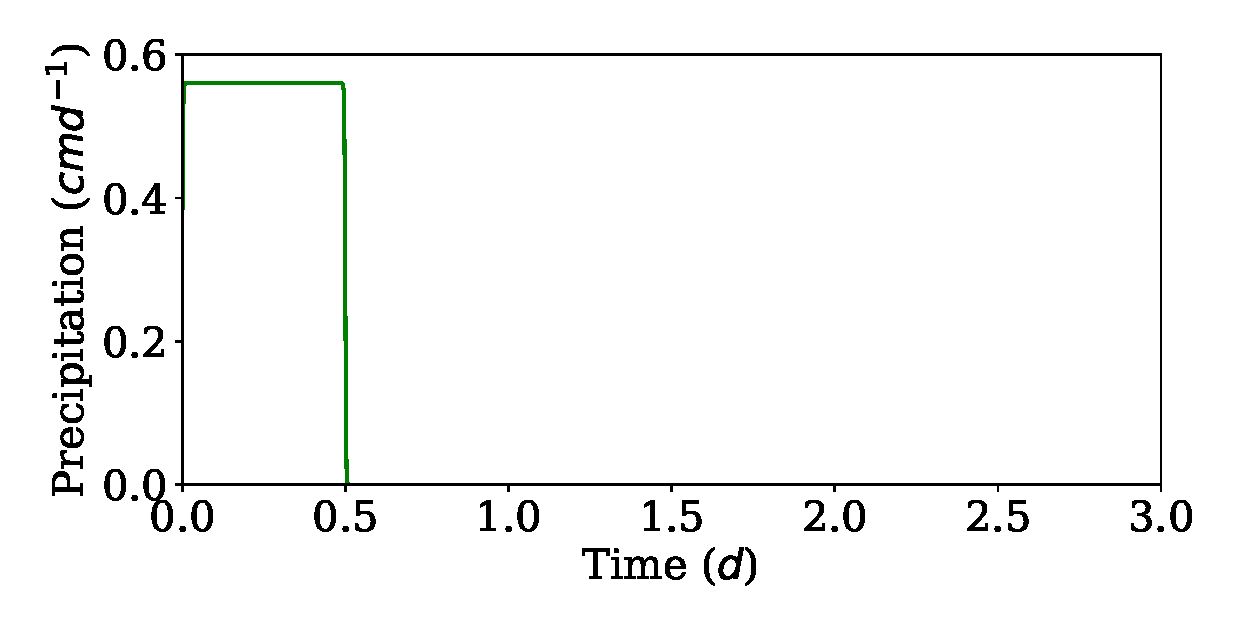
\includegraphics[width = \linewidth, keepaspectratio] {pr_ppat1ptot0_28.eps}
		\caption{}
	\end{subfigure}
	\begin{subfigure}{0.32\textwidth}
		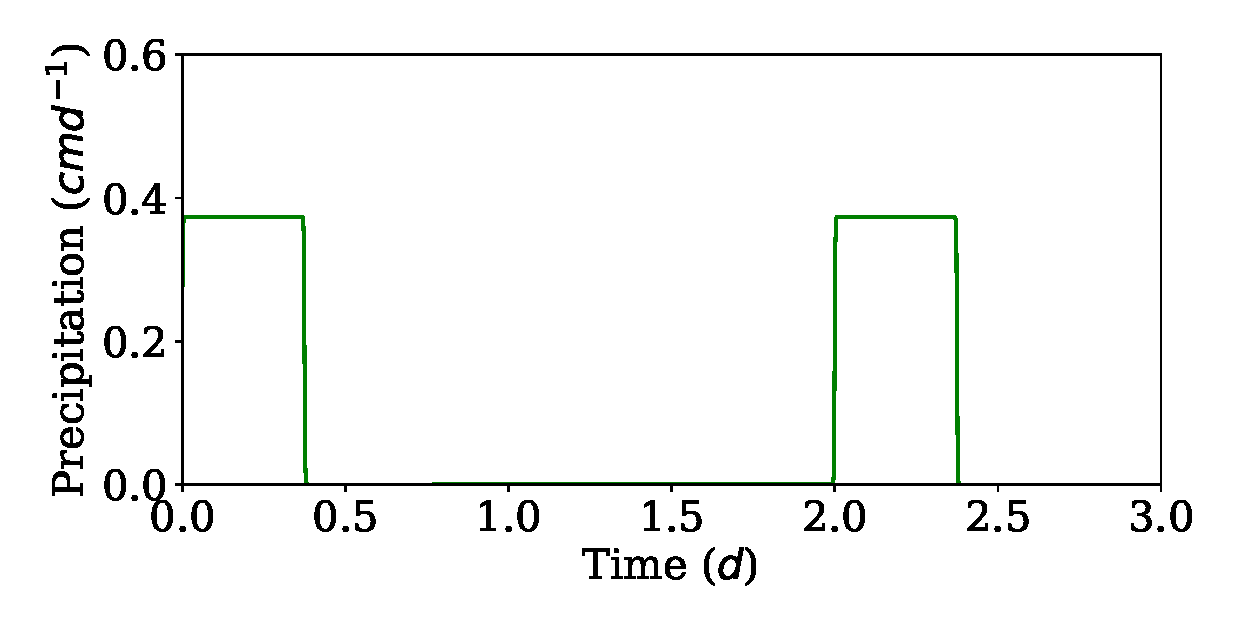
\includegraphics[width = \linewidth, keepaspectratio] {pr_ppat2ptot0_28.eps}
		\caption{}
	\end{subfigure}
	\begin{subfigure}{0.32\textwidth}
		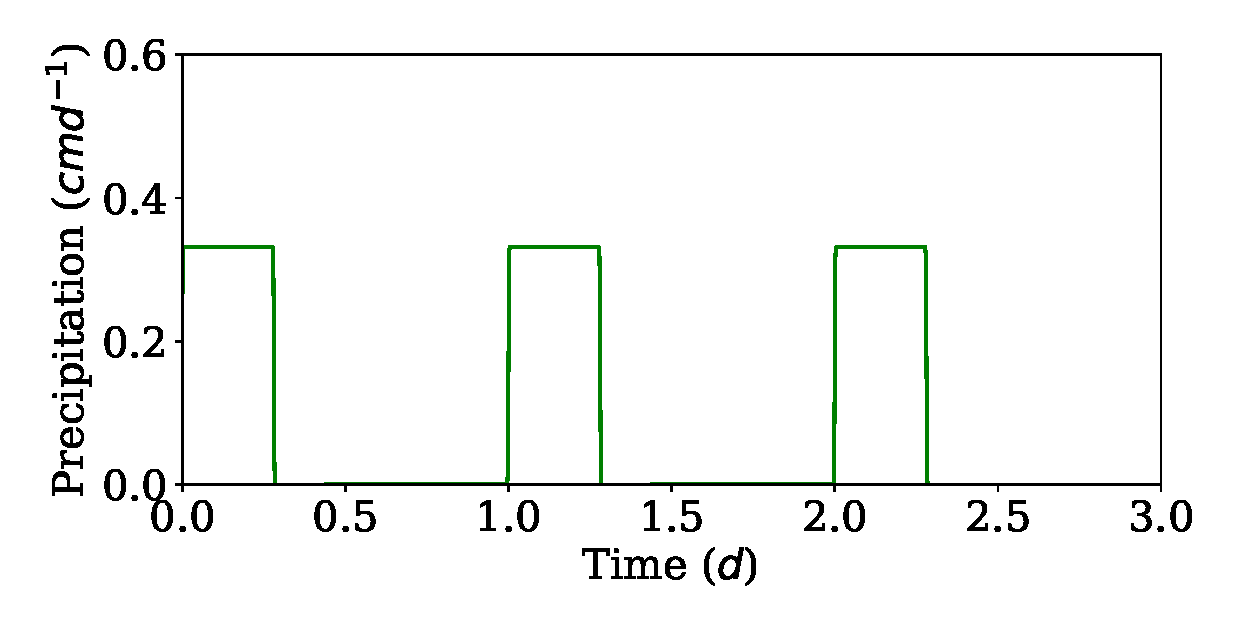
\includegraphics[width = \linewidth, keepaspectratio] {pr_ppat3ptot0_28.eps}
		\caption{}
	\end{subfigure}\\
	\begin{subfigure}{0.32\textwidth}
		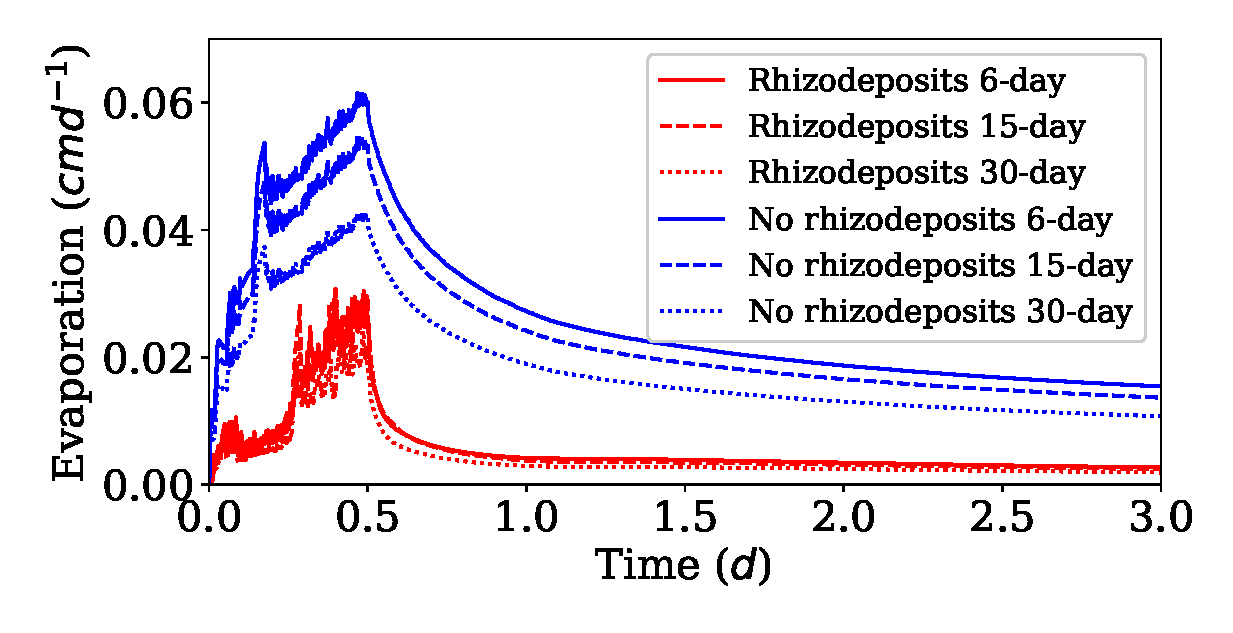
\includegraphics[width = \linewidth, keepaspectratio] {ev_ppat1ptot0_28.eps}
		\caption{}
	\end{subfigure}
	\begin{subfigure}{0.32\textwidth}
		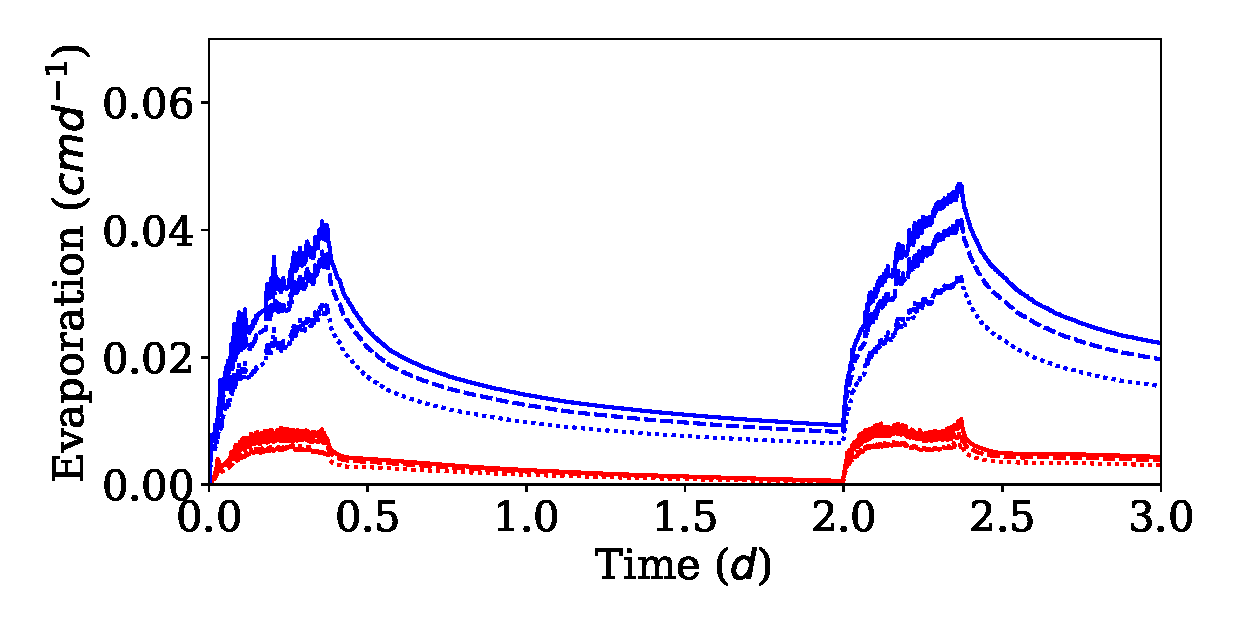
\includegraphics[width = \linewidth, keepaspectratio] {ev_ppat2ptot0_28.eps}
		\caption{}
	\end{subfigure}
	\begin{subfigure}{0.32\textwidth}
		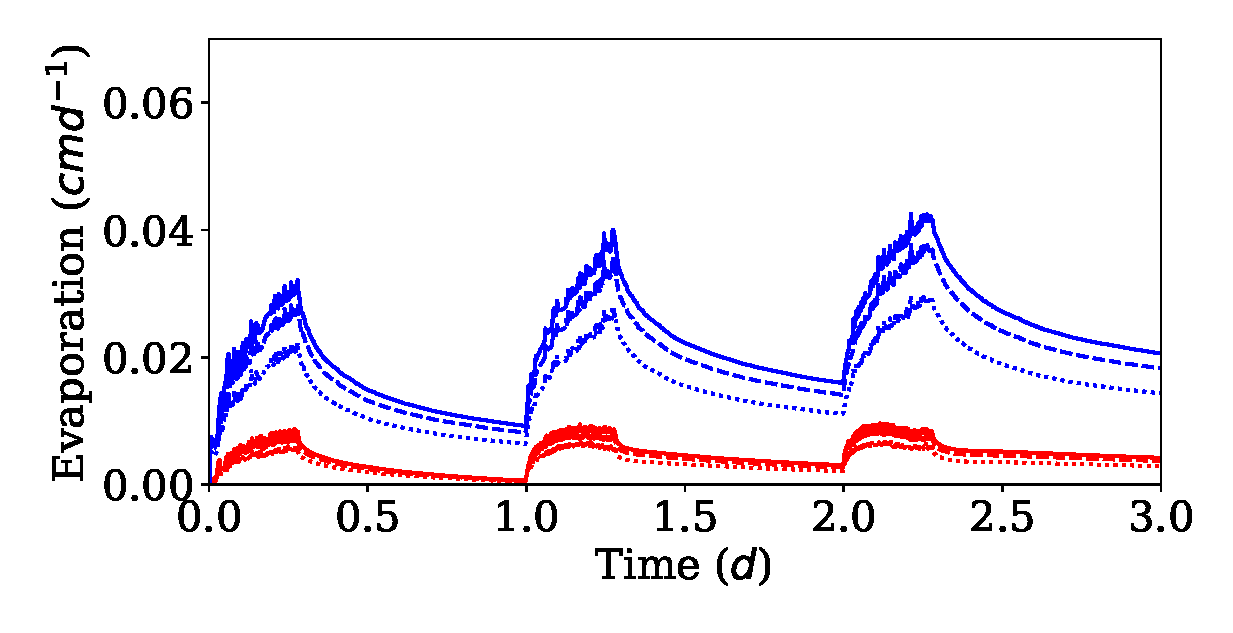
\includegraphics[width = \linewidth, keepaspectratio] {ev_ppat3ptot0_28.eps}
		\caption{}
	\end{subfigure}\\
	\begin{subfigure}{0.32\textwidth}
		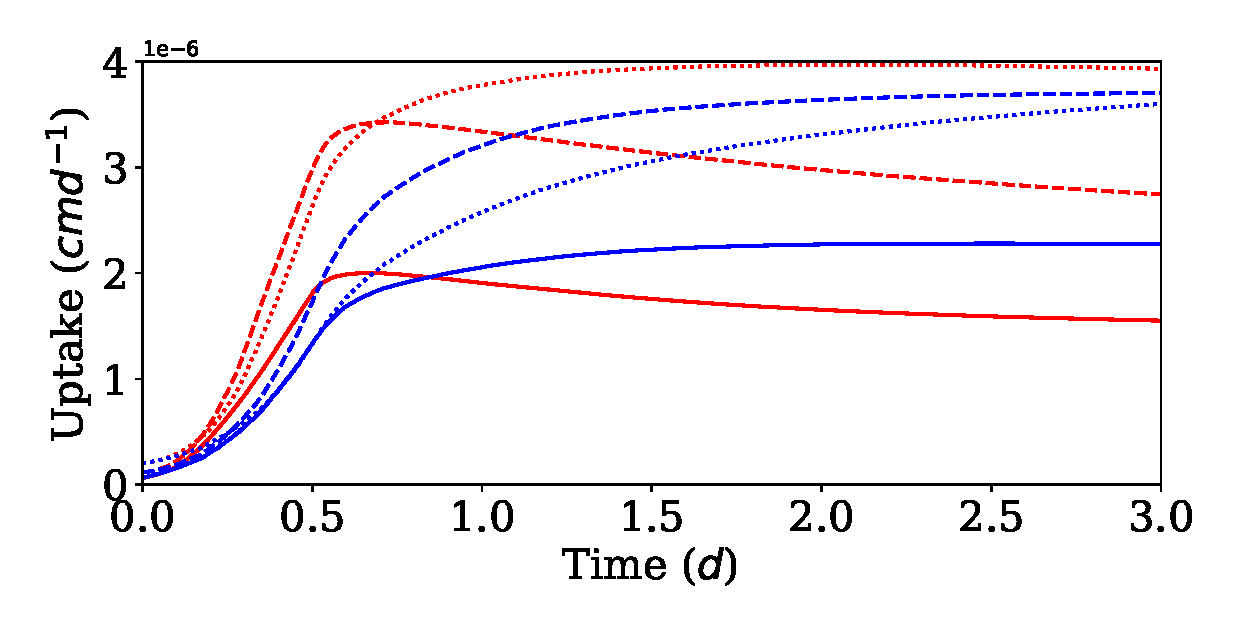
\includegraphics[width = \linewidth, keepaspectratio] {up_ppat1ptot0_28.eps}
		\caption{}
	\end{subfigure}
	\begin{subfigure}{0.32\textwidth}
		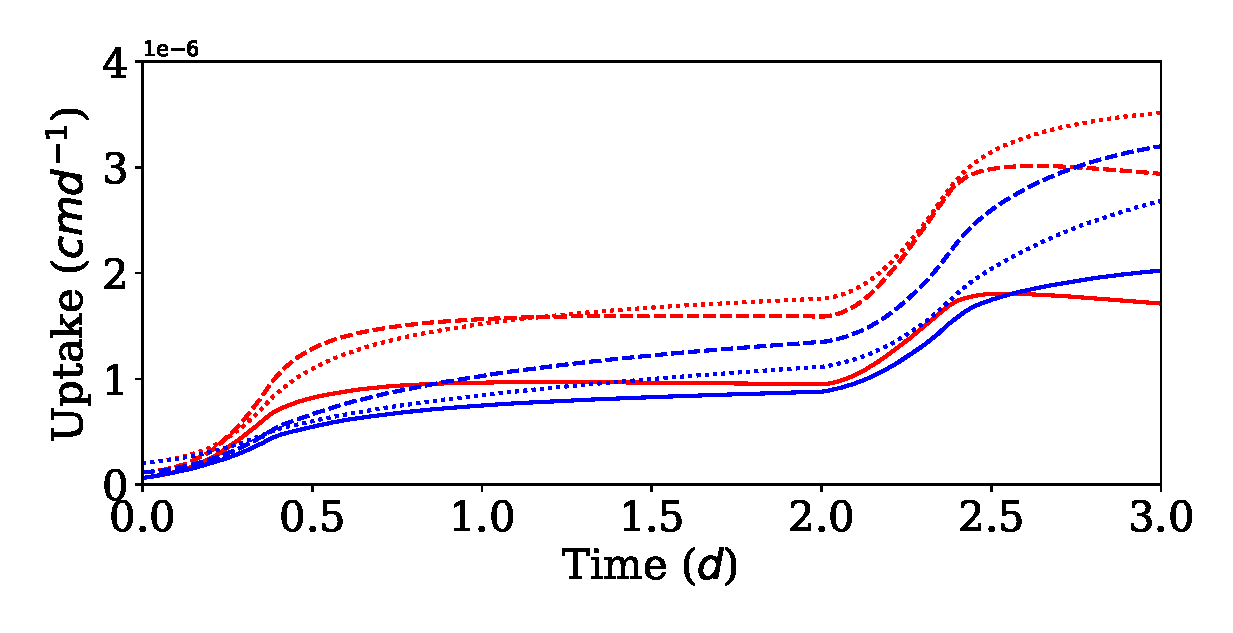
\includegraphics[width = \linewidth, keepaspectratio] {up_ppat2ptot0_28.eps}
		\caption{}
	\end{subfigure}
	\begin{subfigure}{0.32\textwidth}
		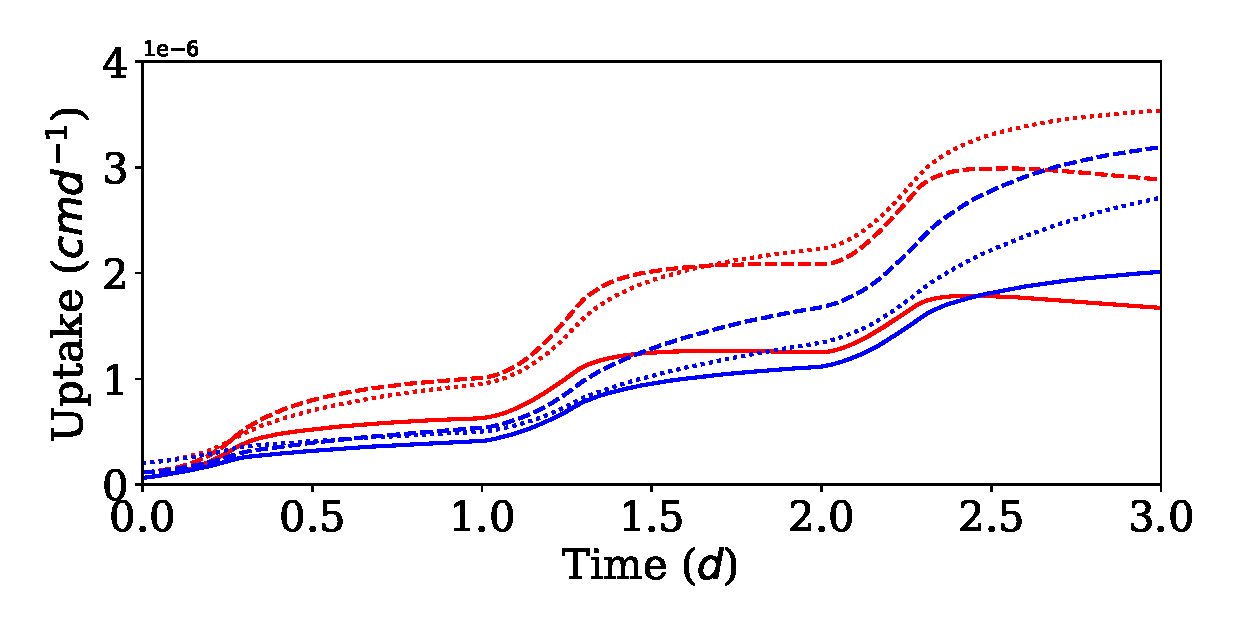
\includegraphics[width = \linewidth, keepaspectratio] {up_ppat3ptot0_28.eps}
		\caption{}
	\end{subfigure}
	\caption{The influence of rhizodeposits on the evolution of soil water content and flux over time under the single-event pattern of the higher total rainfall regime. The figures of the leftmost column shows the normalised root length density profiles of each plant with age increasing downwards. The remaining columns show snapshots of the water content dynamics (with and without rhizodeposits) at different time points of the simulation where each row relates to soil vegetated by the roots of each age of plant. The arrows illustrate the strength of the flow at each time point of the various conditions}
	\label{figure: Madrid_precip_evap_up}
\end{figure}

\begin{table}
	\centering
	\smaller
	\begin{tabular}{{ |p{3cm}||p{1.55cm}|p{1.55cm}|p{1.55cm}|p{1.55cm}|p{1.55cm}|p{1.55cm}||}}
		\hline
		\multicolumn{1}{|l||}{Total rainfall} &
		\multicolumn{6}{|c||}{0.28cm}\\
		\hline
		\multicolumn{1}{|l||}{Rainfall distribution} &
		\multicolumn{2}{|c|}{1 event} &
		\multicolumn{2}{|c|}{2 events} &
		\multicolumn{2}{|c||}{3 events}\\
		\hline
		Rhizodeposits & No & Yes & No & Yes & No & Yes\\
		\hline
		Total uptake: 6-day old plant (cm)& $5.66\times10^{-6}$ & $4.71\times10^{-6}$ & $2.88\times10^{-6}$ & $3.19\times10^{-6}$ & $2.86\times10^{-6}$ & $3.22\times10^{-6}$\\
		\hline
		Total uptake: 15-day old plant (cm)& $8.85\times10^{-6}$ & $8.25\times10^{-6}$ & $4.22\times10^{-6}$ & $5.23\times10^{-6}$ & $4.18\times10^{-6}$ & $5.26\times10^{-6}$\\
		\hline
		Total uptake: 30-day old plant (cm)& $7.83\times10^{-6}$ & $1.01\times10^{-5}$ & $3.49\times10^{-6}$ & $5.47\times10^{-6}$ & $3.49\times10^{-6}$ & $5.52\times10^{-6}$\\
		\hline
	\end{tabular}
	\caption{Total uptake of each root system with and without rhizodeposits for each rainfall distribution of the higher-rainfall regime.}
	\label{table: higher rainfall total uptake}
\end{table}

\begin{figure}
	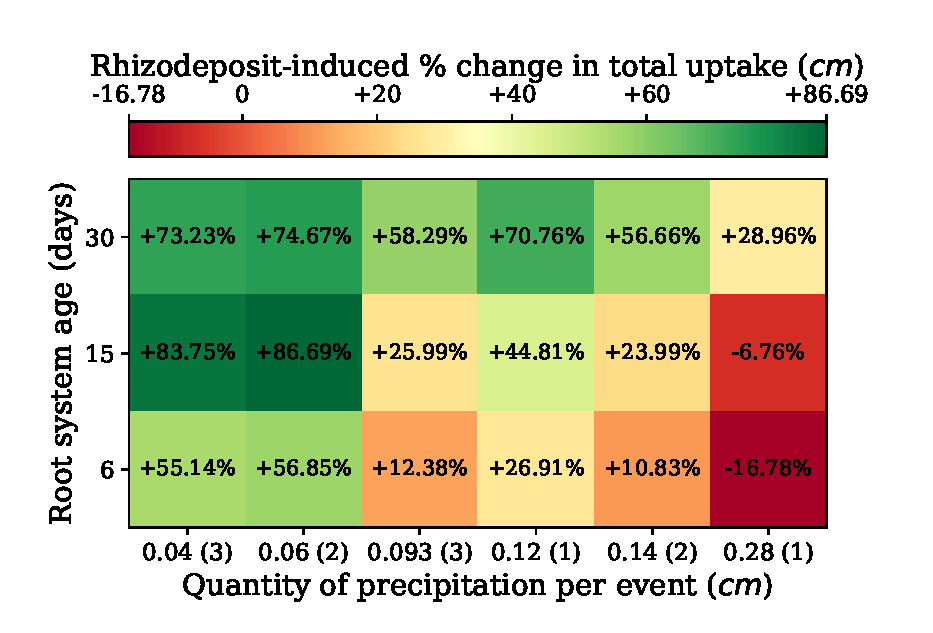
\includegraphics[width = 1.0\linewidth, keepaspectratio]{age_vs_rain_per_event.eps}
	\caption{The strength of the positive or negative effect of rhizodeposits on total water uptake of a root system in relation to root system age/depth and the quantity of precipitation delivered in each rainfall event of the precipitation regime.}
	\label{figure: uptake_age_intensity}
\end{figure}

\section{Discussion}

\subsection{Future incorporation of rhizodeposit influence in models of soil hydraulics: consolidation and calibration}
Within the field of mathematical modelling, there are differing approaches to address rhizodeposit influence on soil hydraulic properties. Like in~\citep{vogel1996hydrus, karagunduz2001influence}, our model assumes that rhizodeposit induced changes to contact-angle and surface tension can be incorporated into the water retention~\eqref{model: water retention} and hydraulic conductivity~\eqref{model: hydraulic conductivity} functions of~\cite{mualem1976new} and~\cite{van1980closed} by using saturated hydraulic conductivity and inverse air entry pressure terms~\eqref{model: saturated hydraulic conductivity},~\eqref{model: alpha vs rhizodeposits} whose values are appropriately scaled according to the abundance of rhizodeposits. Similarly, \cite{landl2021modeling} described mucilage effects on hydraulics by using the approach of~\cite{kroener2014nonequilibrium}, where pressure head with respect to water content is instead modelled by adding a shift term to the function of~\cite{mualem1976new} and~\cite{van1980closed}, which depends on mucilage and rhizosphere bulk density, and by scaling the saturated hydraulic conductivity by a term that depends on the viscosities of water and mucilage. This was not the case, however, in~\citep{cooper2017fluid, cooper2018effect}, where the influence of root exudates was incorporated into Richards equation through a rigorous multi-scale derivation, and the effect of increasing contact angle resulted in retention and conductivity curves that did not result the commonly used functions of~\cite{brooks1964hydrau} or~\cite{mualem1976new} and~\cite{van1980closed}. 

There are also a number of approaches to accounting for root water uptake in models for soil water transport. One approach is to simultaneously model water flow within the root system as well as the soil, with a boundary condition in which the passage of water is driven by pressure differences between the two domains~\citep{gardner1991modeling, javaux2008use}. For simulations over longer time periods and at larger scales, the computational demands of this approach are prohibitive, and attempts have since been made to develop uptake sink terms that allow cheaper simulation of Richards equation but still account for hydraulics within the root system~\citep{couvreur2012simple}. 

In this work, a more classical macroscopic approach~\citep{vsimuunek2009modeling} was taken to incorporate root water uptake into the model for rhizodeposit-influenced soil water transport~\eqref{model: water transport}. Here the uptake function~$S$ integrates over the soil domain to give the transpiration rate of the plant, with adjustments made for local soil water stress. The potential contribution to this transpiration rate from each region of the soil domain is weighted according to the normalised root length density function~$NRLD$, and~$NRLD$ is formulated so that, for any root system, it integrates to 1 over the entire soil domain. Results show (Figures~\ref{figure: almeria_precip_evap_up},~\ref{figure: Madrid_precip_evap_up} and Tables~\ref{table: lower rainfall total uptake},~\ref{table: higher rainfall total uptake}) that this particular property could lead to anomalies when comparisons are made between uptake performance of root systems of different size. This is because for smaller root systems the vegetated region of the domain, where the~$NRLD$ function takes non-zero values, will be smaller. Hence, in order to have a unit integral over the soil, these~$NRLD$ functions of smaller root systems reach larger maximum values than those corresponding to more mature root systems who take non-zero values over a greater portion of the domain. Therefore, if the transpiration rate of the larger root system is not set to a value that is sufficiently greater than that of the smaller root system, then, assuming equal water availability, the smaller root system will have the capacity to reach greater uptake rates than the larger one. In our model, the transpiration rate associated to each root system increases with age in accordance with data on basal crop coefficients~\citep{allen1998crop}. However, this increase is not enough to counteract the anomalous effect of the use of a normalised root length density function and, under the conditions of more intense rainfall with no rhizodeposits to boost the downward flow of water, uptake rates and total uptake are greater for the 15-day old root system than the 30-day old one. This feature of the macroscopic approach means that model~\eqref{model: water transport} may generally underestimate the uptake of larger root systems. If continuing with macroscopic $NRLD$-based uptake terms going forward, then the transpiration rates in~$S$ need to be formulated so that their maturity-related increases are explicitly dependent on root system biomass. 


The potential drawbacks among the range of possible approaches, as well the fact that many model parameters often have to be taken from a wide range of existing publications~\citep{landl2021modeling, mair2023can, mair2022model} indicate the challenges in reliably calibrating and applying models to study the effect of rhizodeposits on soil hydraulics and root water uptake. Future work is needed to consolidate the approach to modelling these processes, which will clarify what data are required for model calibration and focus the design of experiments that are carried out to obtain them.

\subsection{Rhizodeposits as a mechanism for facilitated water infiltration}
Many studies have found that the presence of roots in soil facilitates water infiltration following precipitation~\citep{cerda1999parent,marshall2014impact,wu2016mixed}. Indeed the hydraulic conductivity of soils vegetated by maize, willow and grass have been observed as higher than their fallow counterparts~\citep{feki2018influence, leung2018plant}. One of the proposed mechanisms behind this is the preferential flow of water through macropores that are created as growing roots, and the fauna that their by-products attract, fragment and rearrange the soil~\citep{angers1998plant,luo2019roots}. Additionally though, rhizodeposits have also been shown to have a surfactant effect when present in the soil water solution~\citep{read1997surface, read2003plant, naveed2019surface} and, since surfactants are often applied in agriculture to aid water infiltration into hydrophobic soils~\citep{ogunmokun2020influence}, there is support for the claim that the facilitated water infiltration observed in vegetated soil can be partly attributed to the effect of certain rhizodeposits. Such an effect is captured within the formulation of our water transport model~\eqref{model: water transport}, where rhizodeposit-induced reductions to surface tension increase the soil hydraulic conductivity and alter the water retention curve so that the downward flux of soil water is facilitated. As a result, in our simulations where rhizodeposits were present, water infiltrated more quickly after the onset of precipitation and the rate of water loss by evaporation was reduced. This concurs with similar experimental results regarding evaporation losses under the application of bio-surfactants~\citep{gutierrez2022investigating}. Our results also highlighted, however, that, with enhanced water infiltration, a clear trade off exists between increases in water availability to the root system through reduced evaporation losses and decreases as a result of more powerful downward drainage. For an interval of time during and after rainfall, the rhizodeposit-induced early arrival of water to the root zone caused a higher uptake rate compared to soils without rhizodeposits. For less intense rainfall events, the gradients in water potential that develop between the more saturated surface and the drier rooted zone are less severe and the total amount of water delivered is smaller. Consequently, the rhizodeposit-facilitated water infiltration remained gradual enough, and the quantities of water arriving early to the uptake zone sufficiently small, that the shallower-rooted 6-day and 15-day old plants could enjoy rhizodeposit-boosted uptake rates for the entire simulation time, and not overly suffer from water bypassing their roots. As the rates of rainfall during each event of our simulations were increased the gradients driving  water flux became greater. Therefore, with time, the added influence of rhizodeposits caused larger quantities of water to more quickly reach greater depths and thus become inaccessible to the root systems of the 6 and 15-day old plants. This explains why, despite an early boost, uptake rates sooner or later dropped below those observed when rhizodeposits were not present~(Figure~\ref{figure: Madrid_precip_evap_up}), and the net effect on total water uptake was negative~(Figure~\ref{figure: uptake_age_intensity}).

Because the 30-day old plant had a deeper root system, when rhizodeposits facilitated the transport of water to greater depths it still remained accessible to the plant. Consequently, the preservation of water form the reduction in evaporation losses outweighed the losses of water in the downward direction, and uptake rates with rhizodeposits were, therefore, consistently higher than if there were no rhizodeposits present.

In summary, the findings of our work suggest that the consequences of water infiltration-facilitating rhizodeposits on plant water uptake may not be universally positive and will depend upon the precipitation or irrigation conditions considered. Specifically, if total precipitation over a given time arrives in fewer more intense events, then the uptake of less developed or naturally shallow root systems may be hindered by excessive surfactant-induced acceleration of downward water transport. This is consistent with knowledge on optimal irrigation practices for soils that exhibit generally high water infiltration rates, where methods that promote more gradual surface water application are promoted in order to avoid losses by leaching~\citep{blackwell2000management, alhammadi2013irrigation}. Nevertheless, in environments where precipitation is less intense and more regular, rhizodeposits that facilitate water infiltration are more likely to improve water availability and have a positive influence on uptake and crop performance~\citep{oostindie2010influence, chaichi2015surfactant}.  

The important qualification to accompany these conclusions, though, is that not all rhizodeposits influence soil hydraulics in the same way. For example, there is evidence of maize, barley and chia increasing the viscosity of soil water solutions~\citep{naveed2019surface}, which would reduce hydraulic conductivity in the rhizosphere and, in contrast to the results of this paper, hinder the movement of water around the root. The characteristics of the rhizodeposits of a given plant species are almost certainly not constant over time. In fact, there is growing evidence that the production rate and chemical profile of rhizodeposits are adaptive to biotic factors like growth stage, and external factors such as soil type and water or nutrient availability~\citep{rolfe2019crying,wen2022linking,williams2020plant}. This, therefore, gives weight to claims that rhizodeposits function to engineer the soil in accordance with needs of the plant, as opposed to being merely a waste product whose potential effects on water and nutrient availability are coincidental.       

\subsection{Harnessing rhizodeposits for the development of crop ideotypes with resilience to enviroment-specific stresses.}
The Green Revolution of the 1960s, with the increased use of chemical fertilisers, pesticides and precise irrigation, shifted the attention of crop breeders towards the question of maximising yield under conditions where stresses from water and nutrient shortages or competition were minimal~\citep{preece2020return}. This approach led to a focus on optimal above ground traits, where one direction was to breed for crops that maximised the ratio of harvestable above ground biomass to total above ground biomass (the harvest index)~\citep{richards1993improving}. Since progress in this aspect rapidly became marginal, improvements to total above ground biomass were then sought and achieved through breeding for rapid leaf area development, to reduce evaporation losses from the soil, and enhanced leaf-level water use efficiency. Within the context of roots, however, the aim of many was to maintain root development at the necessary minimum so as to maximise resource allocation to harvestable biomass under ideal growing conditions~\citep{condon2004breeding}. Latterly, though, with the increasing incidence of global drought, breeding strategies for resilient crops have come to consider more developed root systems with features to improve access to soil water. 

Genes have been identified that control gravitropic response and radial growth~\citep{hafeez2024breeding} and there is a belief that increasing rooting depth should be the target of breeders. This is firstly because it allows rain-fed crops to access deep stores of water during periods of drought~\citep{lynch2013steep, uga2013control}, and secondly because, in wheat systems specifically, root arrival at deep water stores tends to coincide with grain-filling season thus boosting pre-harvest biomass~\citep{palta2011large, wasson2012traits, ober2021wheat}. Evidence has also been shown of a genome effect on rhizodeposit and microbiome features~\citep{iannucci2021relationships}, and it has been tentatively proposed that crops could be bred to promote the development of microbiomes that are specifically beneficial under certain stresses~\cite{ober2021wheat}. 

One problem with this, however, is that it is far from easy to verify that a given crop genotype induces the microbiome characteristic it has been purported to. Interactions between root rhizodeposits and other actors in the microbiome are complex and vary in nature at the different stages of plant growth~\citep{bakker2012harnessing,oburger2018sampling}. Furthermore, non-destructively extracting rhizodeposits from roots grown in the field is massively challenging, and, when taking the more simple approach of extracting from roots grown in hydroponic systems, it cannot be guaranteed that the same rhizodeposit properties would be observed for roots grown in soil~\citep{oburger2018sampling}. Another challenge with selecting stress-resilient ideotypes based on rhizodeposit characteristics is determining their effect on macroscopic agricultural outputs. For instance, the findings of this article suggest that when rhizodeposits have a chemical composition that makes them act as surfactants, they can reduce evaporation losses from the soil and improve the uptake performance of deeply rooted systems. But, due to a lack of consensus regarding the correct modelling approach and limitations regarding accurate parametrisation, the insights that can be drawn from results like these are modest and, at present, cannot realistically be incorporated into large scale models for crop performance and yield. Because of issues like these, few breeding programmes currently incorporate rhizodeposit characteristics in there selections~\citep{preece2020return}. For this to change, technological advances will be required to improve the viability of experiments involving rhizodeposits, and the modelling community must establish a greater consensus on how rhizodeposit effects on soil hydraulics should be incorporated into models across all scales, but particularly those used in agricultural practice.

%\begin{figure}
%	\centering
%	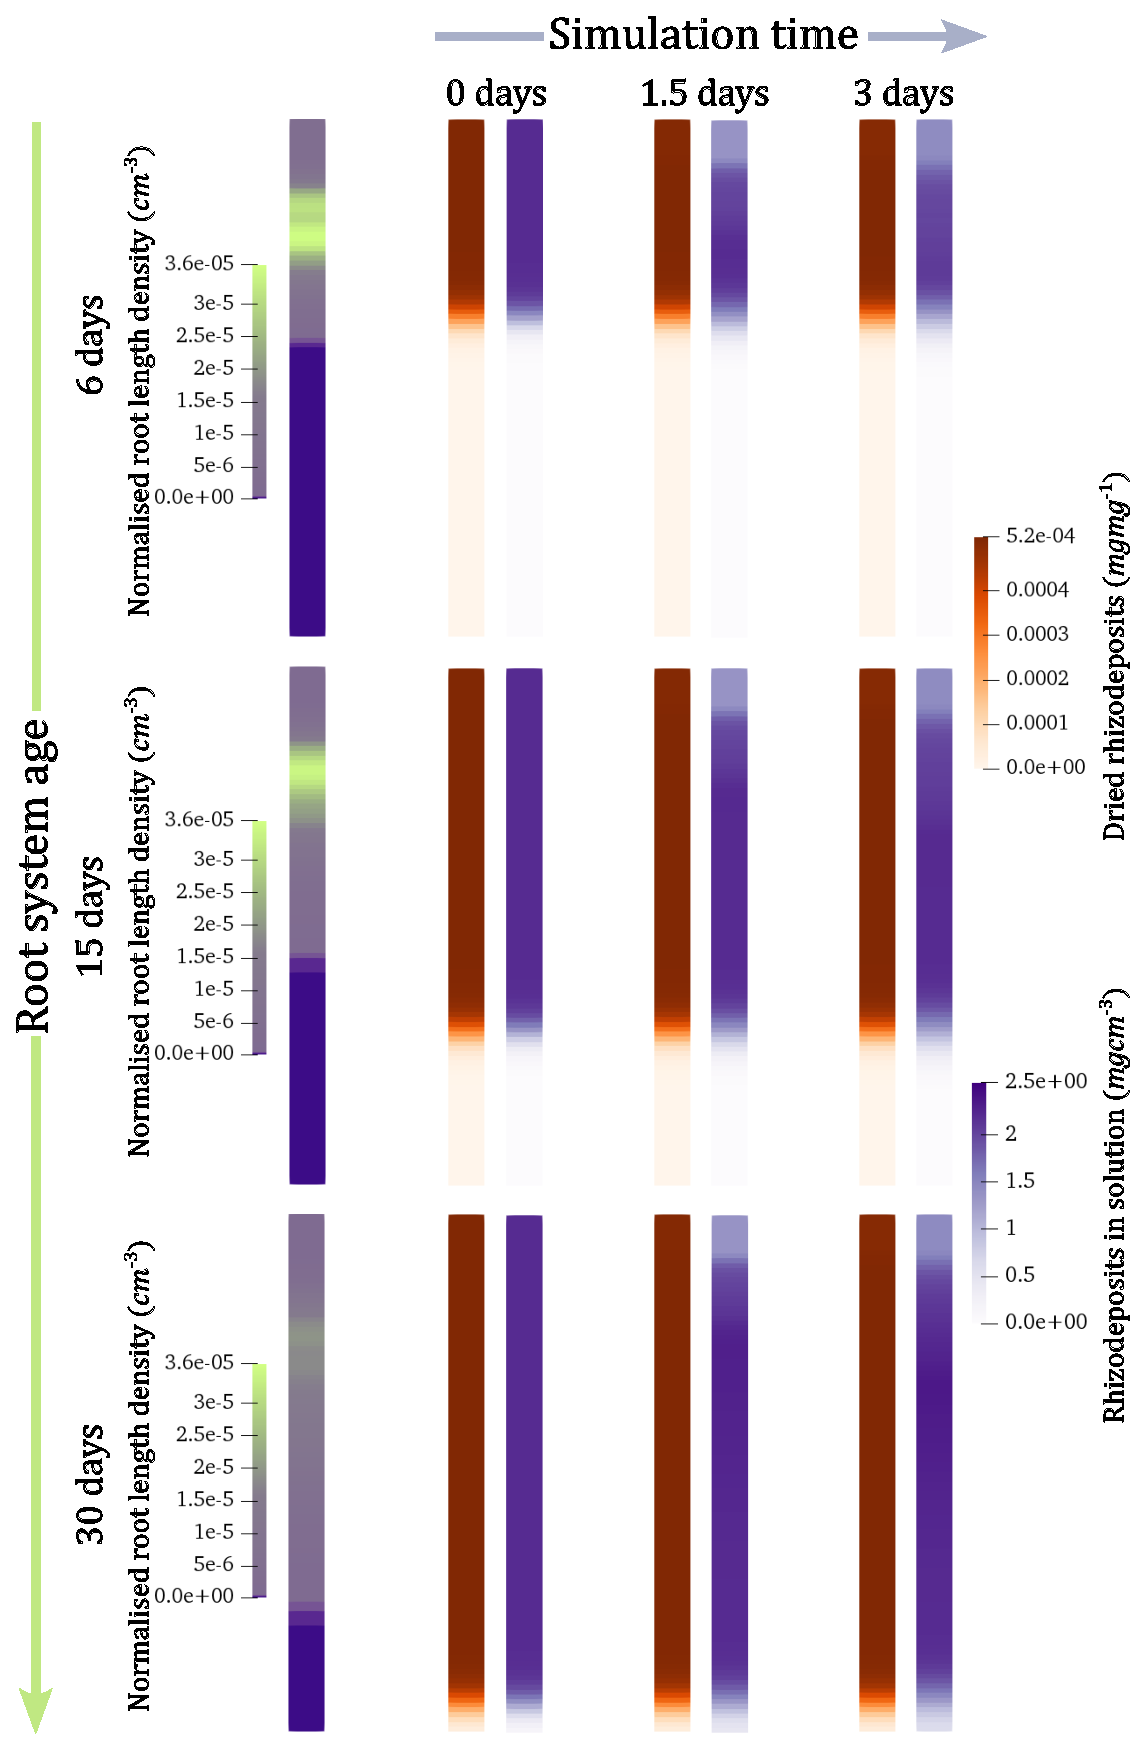
\includegraphics[width = 0.75\linewidth, keepaspectratio]{rhizodeposit_profiles_almeria_3_events.eps}
%	\caption{Almeria rhizodeposits}
%	\label{figure: almeria_3_events_rhizodeposits}
%\end{figure}
%
%\begin{figure}
%	\centering
%	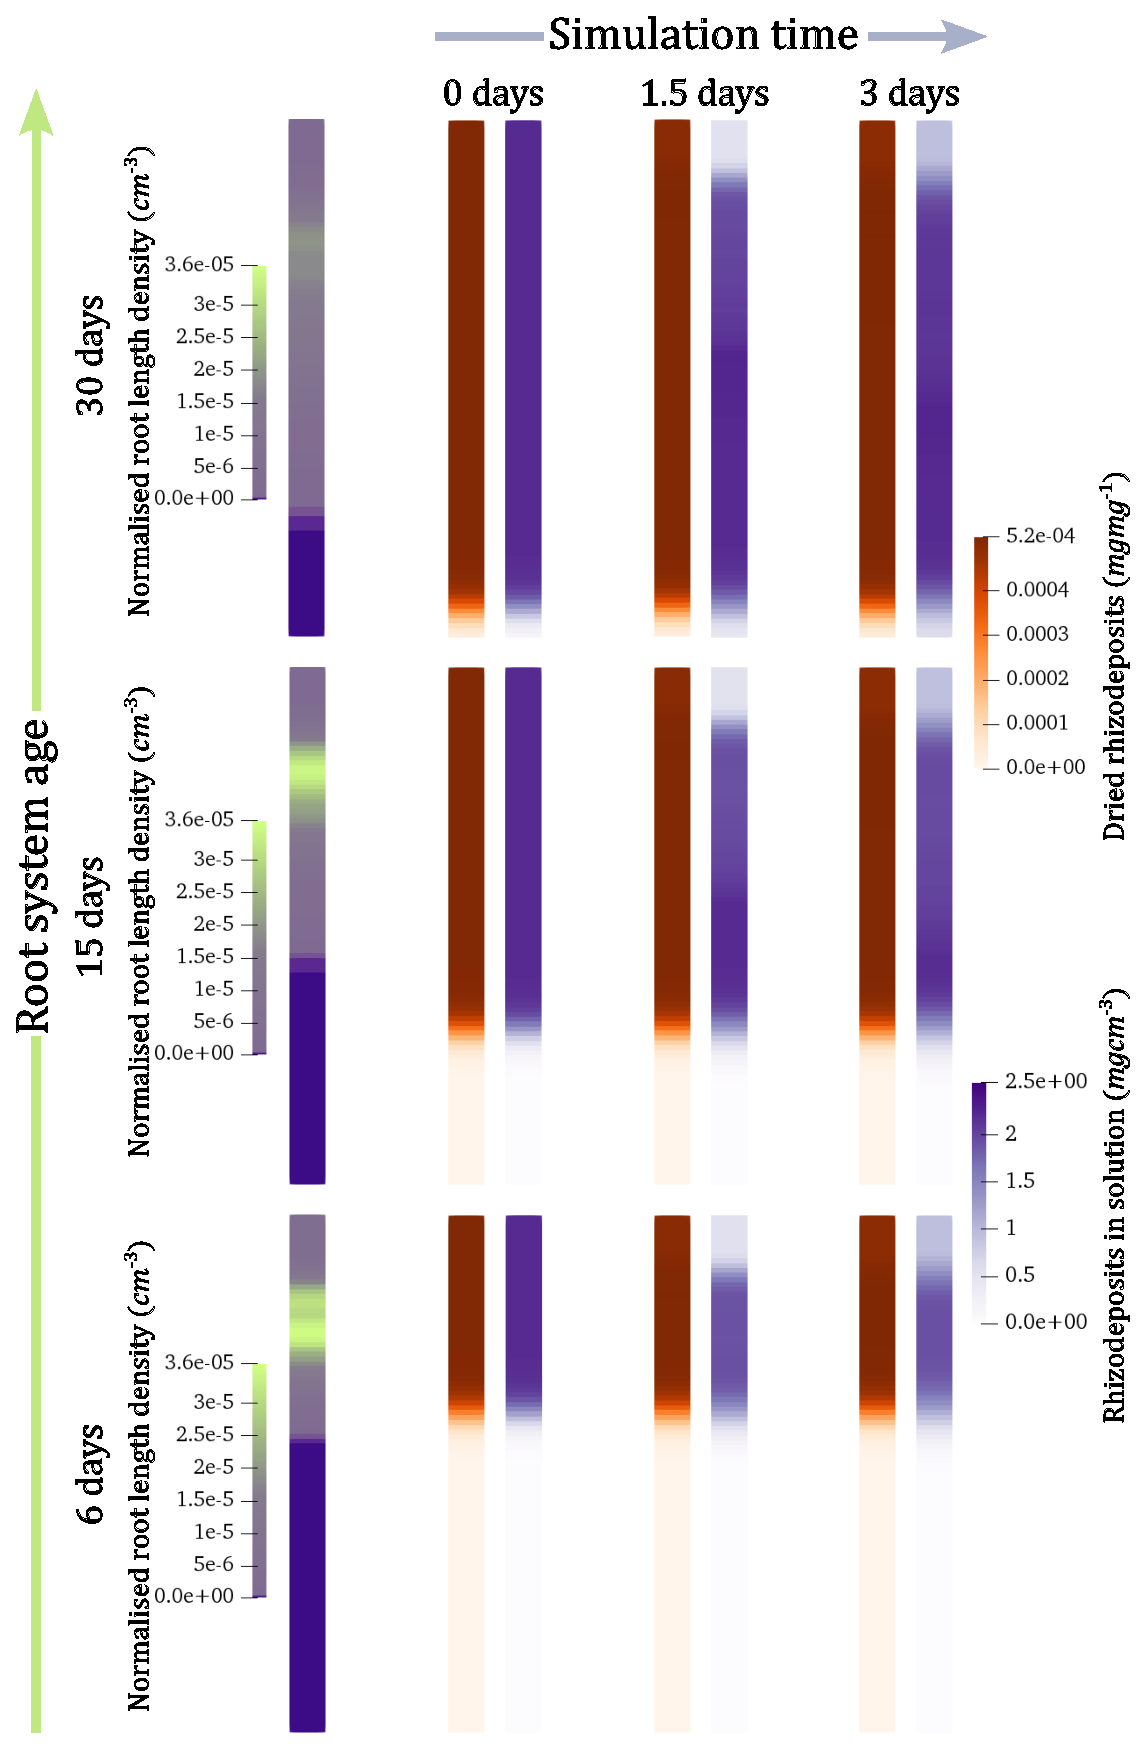
\includegraphics[width = 0.75\linewidth, keepaspectratio]{rhizodeposit_profiles_madrid_1_event.eps}
%	\caption{Madrid rhizodeposits}
%	\label{figure: madrid_1_event_rhizodeposits}
%\end{figure}

\bibliographystyle{chicago}
\bibliography{rhizodeposit_influence_bibliography}

\end{document}	